\documentclass[utf8]{FrontiersinHarvard} % Frontiers in Artificial Intelligence uses the Harvard (author-date) reference style
\usepackage{url,hyperref}
% pagewise (not running) line numbering: avoids the severe slowdown/timeout that
% \linenumbers in running mode causes when combined with many two-column floats
% (figure*/table*) on resource-constrained compile servers.
\usepackage[pagewise]{lineno}
\usepackage[onehalfspacing]{setspace}
\usepackage{algorithmic}
\usepackage{algorithm}
\usepackage{textcomp}
\usepackage{booktabs}
\usepackage{grffile}
\usepackage{float}
\usepackage{placeins}
\def\BibTeX{{\rm B\kern-.05em{\sc i\kern-.025em b}\kern-.08em
    T\kern-.1667em\lower.7ex\hbox{E}\kern-.125emX}}

\linenumbers

% FrontiersinHarvard.cls enters two-column mode via a bare \twocolumn command rather
% than the standard class-option mechanism, so \columnwidth (and \linewidth) never get
% halved for single-column figure sizing -- they stay equal to \textwidth. Any figure
% sized relative to \columnwidth therefore silently requests near full-page width,
% which for a portrait image is tall enough to never fit a column, leaving it stuck in
% the deferred-float queue for the rest of the document (and dragging later floats down
% with it) -- a major cause of runaway compile times. Use this corrected length instead.
\newlength{\truecolumnwidth}
\setlength{\truecolumnwidth}{0.5\dimexpr\textwidth-\columnsep\relax}

% Framework name macro — change once, updates everywhere
\newcommand{\sadrift}{FedSA-Drift}

% Tighter and more stable float placement in two-column layout.
\setcounter{topnumber}{5}
\setcounter{bottomnumber}{5}
\setcounter{totalnumber}{10}
\renewcommand{\topfraction}{0.95}
\renewcommand{\bottomfraction}{0.95}
\renewcommand{\textfraction}{0.05}
\renewcommand{\floatpagefraction}{0.85}
\setlength{\textfloatsep}{10pt plus 2pt minus 2pt}
\setlength{\floatsep}{8pt plus 2pt minus 2pt}
\setlength{\intextsep}{8pt plus 2pt minus 2pt}

\def\keyFont{\fontsize{8}{11}\helveticabold }
\def\firstAuthorLast{Koirala {et~al.}} %use et al only if is more than 1 author
\def\Authors{Apurba Koirala\,$^{1}$, Rajeshkannan Regunathan\,$^{1,*}$ and RA K Saravanaguru\,$^{1}$}
% Affiliations should be keyed to the author's name with superscript numbers
\def\Address{$^{1}$School of Computer Science and Engineering, Vellore Institute of Technology, Vellore, Tamil Nadu, India}
% The Corresponding Author should be marked with an asterisk
\def\corrAuthor{Rajeshkannan Regunathan}

\def\corrEmail{rajeshkannan.r@vit.ac.in}

\begin{document}
\raggedbottom
\onecolumn
\firstpage{1}

\title[FedSA-Drift]{FedSA-Drift: Structure-Aware Drift-Regularized Federated Vision Transformers for Multimodal Skin Lesion Classification Under Heterogeneous Clinical Distributions}

\author[\firstAuthorLast ]{\Authors}
\address{}
\correspondance{}

\extraAuth{}

\maketitle

\begin{abstract}
By using federated learning, healthcare organizations can work together to train their machine learning models with medical records while protecting patient privacy. In addition, federated learning supports compliance with privacy regulations such as GDPR and HIPAA, while enabling multi-institutional collaboration on heterogeneous medical data without sharing raw records. The diversity in the medical data collected by different organizations often leads to heterogeneity between clients, which can cause a number of challenges during the training process, including client drift, unstable convergence, and fairness issues. These challenges can become more pronounced when training on multimodal medical data, where structured clinical metadata is combined with high-capacity Vision Transformer models. This paper proposes a framework called \sadrift{} (Structure-Aware Drift-Regularized Federated Learning) for classifying skin lesions using multimodal medical data. \sadrift{} features a SwinV2-Base backbone fused with structured metadata, and it separates the parameters into three different categories: early vision layers, deeper Transformer layers, and client-specific multimodal heads. The framework also introduces a drift-aware inverse-distance aggregation method to reduce client divergence, without modifying local objectives or adding any additional hyperparameters. Using the ISIC 2019 dataset for testing, centralized training produced an overall balanced accuracy of 0.8867. Under near-IID conditions ($\alpha = 1.0$, $K = 3$), federated learning retained over 93\% of the centralized accuracy. Under moderately heterogeneous conditions ($\alpha = 0.5$, $K = 5$), the worst-client accuracy of FedAvg was only 0.4800. \sadrift{} improved this to 0.5705 and reduced inter-client variance by approximately 39\% in a single experimental trial, with minimal computational overhead. These proof-of-concept results suggest improved stability and fairness for multimodal Vision Transformer models in federated medical imaging, within the tested scope of two client counts and two heterogeneity levels on a single dataset.

\tiny
 \keyFont{ \section{Keywords:} client drift, federated learning, heterogeneous data, medical image analysis, multimodal learning, non-IID data, skin lesion classification, Vision Transformer}
\end{abstract}

\section{Introduction}
\label{sec:introduction}
Melanoma is responsible for a disproportionate number of deaths from skin cancer. It is one of the most common cancers in the world \citep{Arnold2022,Hay2014}. To improve patient outcomes, early and accurate diagnosis is a must. Automated classification of skin lesions using dermoscopic images has greatly improved recently. Much of this improvement has been accomplished through deep learning and large-scale vision models such as Vision Transformers \citep{Naeem2025}.

However, most highly effective models currently rely upon centralized environments where the model is created by pooling all of the data into one single repository. This assumption rarely applies to clinical environments, since due to extremely strict privacy laws and institutional policies, medical data is complex to share across hospitals. The CCPA and the GDPR both limit the direct ability to share the raw data collected by hospitals. Therefore, the laws that restrict the sending of data make multi-institutional collaborations for various medical purposes legally and ethically complex \citep{Voigt2017,Law2023}.

Federated learning (FL) is an alternative to this issue. Institutions can share model parameters with each other, but not their raw data. This allows multiple institutions to collaborate without sacrificing patient privacy \citep{McMahan2017,Rieke2020}. Nevertheless, FL has one major challenge in the medical realm: there is heterogeneity in the data from different hospitals. Medical data in the real world is not independently and identically distributed (that is, non-IID). All of the differences in patient demographics, the number of patients with a certain disease, the imaging devices and device settings used to image patients (metadata) all contribute to statistical heterogeneity in the datasets \citep{Zhao2018,Li2020}.

The complexity of multimodal learning tasks compounds the challenge. Analysis of skin lesions, for example, requires both imaging as well as clinical metadata which includes age, gender and anatomical location \citep{Nunnari2020,Gessert2020}. When done in a centralized setting, patient metadata typically increases diagnostic performance. Patient metadata contains information about the clinical context that cannot be derived from visual features only \citep{Gessert2020,Nunnari2020}.

The aggregation of multimodal data creates additional challenge due to heterogeneity when utilizing federated systems. Image distributions alone are already heterogeneous among various healthcare institutions due to many differences between imaging devices and patient characteristics. When considering the distribution of metadata, it is much more heterogeneous than image distributions. For example, within a paediatric clinic, there may be significant representation of a constrained age range. In a specialist centre or referral clinic, there may be substantial representation of only one or very few anatomical sites. The manner in which sex and body location are recorded may also vary across electronic health record systems. Thus, fusing two heterogeneous modalities and distributing them across clients through a shared model only serves to further exacerbate instability. Therefore, client drift is exacerbated in multimodal federated systems compared with those only containing imaging \citep{Zhu2025}.

The aggregation of all model parameters uniformly is not appropriate for multimodal architectures. The visual backbone of a model and the metadata fusion component perform different tasks within a model, and each modality may be subject to varying distributions among each of the clients. If these two different modalities are aggregated in the same manner, the visual representation will be corrupted. Likewise, the metadata components will not be allowed to acclimate or adapt to local institutional characteristics \citep{Zhu2025}. Therefore, in order to build a stable and equitable multimodal federated system, client drift must be addressed and the structural differences between model components must be respected. Figure~\ref{fig:intro_federated} illustrates this federated setup.

\begin{figure}[htbp]
\centering
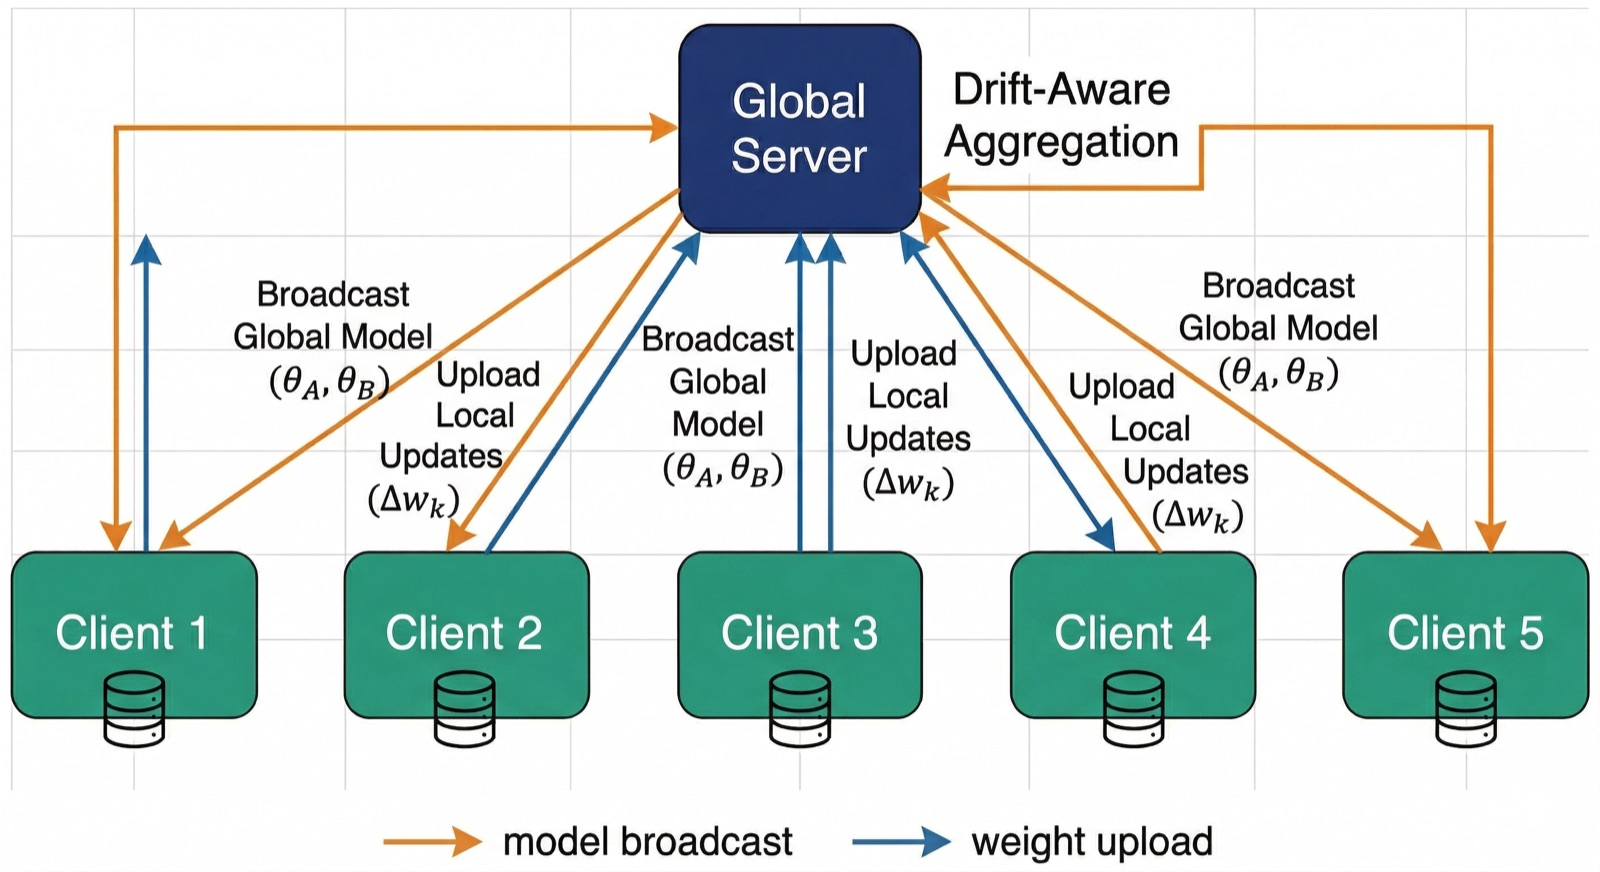
\includegraphics[width=0.82\truecolumnwidth]{images/Intro.jpg}
\caption{Overview of the federated learning setup with 5 clients. Each client trains locally on private data and uploads model updates to the global server. The server aggregates updates via drift-aware inverse-distance weighting and broadcasts the updated global model parameters back to all clients.}
\label{fig:intro_federated}
\end{figure}

\subsection{Existing Solutions and Limitations}

Federated Averaging (FedAvg) is the de facto standard for federated optimization algorithms \citep{McMahan2017}. It averages the models from all clients weighted according to the size of the local dataset for each client. The FedAvg algorithm works well when local data distributions are similar to one another. However, when data is non-IID, the local models begin to drift; this means that the local models will converge toward different optimal points, resulting in a biased or unstable aggregate model \citep{Karimireddy2020,Li2020}.

Different methods have been proposed to address this problem. There are proximal regularization methods that introduce a penalty to any local update that deviates from the global model \citep{Li2020}. Alternatively, there are also methods that use control variates or partial personalization strategies \citep{Karimireddy2020,Collins2021}. However, using these additional methods typically requires the introduction of additional hyperparameters or a modification of the objectives that are normally employed to train local models.

For multimodal federated learning, the majority of approaches consider the model a single set of parameters. That is, all layers of all models are aggregated in the same way, regardless of the role of each layer. This does not take into account that the early feature extractors and the deep semantic layers will behave very differently under any change in distribution. As a result, uniform aggregation produces instability in shared representations and limits the ability of institutions to specialize \citep{Zhu2025}.

In addition to this, many researchers and practitioners tend to focus on global metrics such as overall accuracy or AUC. For clinical applications, however, global performance alone is not adequate. For example, a model that performs well on average, but fails at one institution, will create inequities and diminish trust \citep{Darzi2024,Li2021}.

\subsection{Research Gap}

There are still critical gaps that exist in federated medical learning despite past progress.

Sensitivity to layer-wise distributional heterogeneity: Compared to the earlier feature extraction layers, the performance of later deep Transformer model layers is more adversely impacted by distributional heterogeneity. Research on federated Vision Transformers indicates that if the multi-head attention remains misaligned across multiple client devices, the performance of the other clients will suffer due to feature collapse \citep{Darzi2024}. Studies evaluating partially personalized models show that uniformly aggregating shared model parameters negatively impacts the device drift experienced by clients \citep{Zhu2025}. Most current methods uniformly aggregate all shared model parameters while failing to take into account the different functional behaviours exhibited by the various layers of the model.

Multimodal personalization: Structured clinical metadata frequently varies greatly across hospitals (e.g., age, gender and body structure) \citep{Nunnari2020}. When using multimodal federated models, if the shared visual and the personalized components of the metadata are not kept separate from each other, the divergence of each will increase, thereby decreasing stability \citep{Zhu2025}. Most current methods do not appropriately enforce a separation between these two components.

Client-level stability under severe non-IID conditions: Individual clients may experience substantial drops in performance under conditions of severe non-IID distributional heterogeneity, even though the global metric remains satisfactory. Recent research on federated Vision Transformers shows that there is a critical requirement for the robustness of the worst client in order to stabilise client performance \citep{Darzi2024,Zhao2025}. The majority of current methods are primarily directed toward achieving a global objective and do not provide a mechanism for optimising worst-case client performance.

Moreover, many of the technical methods used to stabilise client performance impose extensive computation costs on client devices, while it is very important that efficiency be considered when developing practical applications for resource-limited environments \citep{Wu2024}. There is therefore a clear need for a federated method that stabilizes critical representation layers and improves fairness without complex local regularization.

\subsection{Objectives}

The objective of this research is to develop a federated multimodal skin lesion classification framework that incorporates the concept of data structure upon which it is designed. Additionally, the framework will be designed with the express intent of being resilient to the different forms of data distribution (heterogeneous data distributions).

This research will accomplish its objectives by developing:


\begin{itemize}
    \item A method to decompose parameters that separates global visual representations from client-specific multimodal heads.
    \item An aggregation mechanism to address client divergence using available data from clients on the server-side.
    \item An examination of how the model behaves under IID versus non-IID conditions, as simulated using a Dirichlet distribution.
    \item A comparison between the performance of federated learning versus the maximum achievable performance of centralized learning.
    \item An evaluation of fairness in terms of worst-case scenario accuracy and inter-client variance for all models.
\end{itemize}

\subsection{Major Contributions}

There are five contributions made by this paper:

\begin{itemize}
    \item \textbf{Structure-Aware Parameter Decomposition:} Model parameters are decomposed in a manner that separates early backbone layers, deep Transformer layers, and client-specific multimodal heads. With this design, the server can selectively aggregate contributions from clients based on the functional role each parameter group plays.

    \item \textbf{Drift-Aware Inverse-Distance Aggregation:} The aggregation mechanism designed for the server-side reduces the overall contribution of outlier clients based on how far they have drifted from prior models. No changes to local training objectives need to be made, nor are any additional regularization hyperparameters required.

    \item \textbf{Proof-of-Concept Heterogeneity Study:} The performance of \sadrift{} was evaluated under near-IID and moderately heterogeneous data distributions using two Dirichlet concentration parameters ($\alpha \in \{0.5, 1.0\}$) and two client counts ($K \in \{3, 5\}$) on the ISIC 2019 dataset. This constitutes an initial empirical characterization; evaluation at larger client counts and more extreme heterogeneity levels is left to future work.

    \item \textbf{Fairness at the Client Level:} The results indicated that worst-performing clients benefited from drift-aware aggregation versus standard FedAvg, while the overall variance between clients was significantly lower.

    \item \textbf{Practical Viability:} The computational overhead incurred by \sadrift{} versus FedAvg was very minor; therefore, it can be practically implemented to facilitate medical-based deployment at multiple institutions.

\end{itemize}

\section{Literature Survey}
\subsection{Survey of Existing Methods}
\subsubsection{Transformer-Based Vision Models}
Automated classification of skin lesions has moved from CNN methods to Vision Transformers (ViTs) that leverage self-attention to capture long-range dependencies. ViTs outperform traditional CNN methods, especially when the class distribution is imbalanced \citep{Aguirre2024}. Hybrid models are now the most common state-of-the-art methods due to their ability to combine local and global features. Strong attention-based fusion models combining ConvNeXt and ViT have produced state-of-the-art performance on ISIC datasets \citep{Naeem2025}. Multi-stream architectures using transformers can extract multi-scale patterns in dermatology \citep{Alshdaifat2025}. Other approaches include segmentation/classification fusion \citep{HyperFusionNet2025}, ensemble models that take into account metadata \citep{HasanRifat2024}, and transformer ensembles that utilize uncertainty as part of the fusion process \citep{Zoravar2024}.
\subsubsection{Skin Lesion Datasets and Benchmarking}
ISIC 2019 and ISIC 2020 are recognized as the standard benchmarks for skin lesion classification because they provide a number of challenges, such as class imbalance, heterogeneous quality of the images, and the presence of out-of-distribution samples. The top-performing methods typically utilize multi-resolution architectures, extensive augmentation of the training data, and a loss function that balances the classes \citep{Gessert2020}. Additionally, incorporating structured demographic information into the classification process increases diagnostic performance \citep{Nunnari2020}. However, the presence of artifacts such as occlusions caused by hair or measurement markers makes the preprocessing of the data more complex \citep{Wegley2026}. Finally, the presence of demographic imbalances in the datasets implies that there may be issues with classification fairness or generalizability \citep{SkinDiversity2024}.
\subsubsection{Federated Learning in Medical Imaging}
Federated Learning (FL) allows for private, cooperative training that meets the GDPR and HIPAA laws \citep{Guan2024}. Initial implementations used small convolutional neural networks that ran Federated Averaging to learn from multiple institutions \citep{Subramanian2025}. By utilizing communication-efficient techniques, such as asynchronous updates at the layer level, the amount of bandwidth required was significantly reduced \citep{Yaqoob2023}. However, there are still issues with data being non-independent and identically distributed (non-IID) between the various participating institutions, and class imbalance exists as well. Dynamic Adaptive Focal Loss is one method of correcting for class imbalance, but it also increases the computational burden and sensitivity to hyperparameters involved \citep{Zhao2025}.
\subsubsection{Federated Vision Transformers}
Federated settings with Vision Transformers create additional computation and communication challenges compared to Federated Convolutional Neural Networks, due in part to their architecture. Strategies to increase efficiency include masking patches during training \citep{Wu2024} and pruning layers in the ViT architecture \citep{Paxton2024}. In addition to being adversely affected by non-IID data, feature collapse is also an issue with Federated ViT learning. Some alignment-based methods have been developed to ensure consistent representation of local and global attention \citep{Darzi2024}. Lastly, personalization and continual learning strategies are being investigated to improve the adaptability of the Federated ViT learning process \citep{Zuo2024,Yao2024}.
\subsubsection{Explainability, Security and System Architectures}
Concerns regarding the robustness, privacy, and interpretability of federated systems have been documented. One way to improve the stability of representations in a federated system is through self-ensembling \citep{Almalik2022}. Techniques for mitigating the effects of adversarial attacks include diffusion-based defenses \citep{Imam2023}. Privacy-preserving techniques, such as random projection, have been suggested as a way to improve communication security between federated clients and providers \citep{Narimani2024}. In multimodal systems, partial personalization leads to better adaptation at the local client; however, it increases the potential for client drift, and thus optimization-based corrections are required \citep{Zhu2025}.
\subsection{Comparative Analysis}
Standalone architectures have consistently been outperformed by hybrid CNN–Transformer models when used in centralized cases \citep{Naeem2025,Alshdaifat2025}. In federated environments, a trade-off exists between model consistency and computational resource efficiency. Alignment-based approaches result in improved model stability but come with a very high overhead cost. Efficiency-based methods reduce the amount of computational resources required to run the models, but at the expense of representational fidelity.
\subsection{Limitations in Prior Work}
\begin{enumerate}
\item \textbf{Client Drift in Heterogeneous Settings:} The client drift phenomenon refers to a non-IID data distribution present in heterogeneous settings, which may cause instability in convergence and thus reduce global performance \citep{Zhu2025}.
\item \textbf{Destructive Efficiency Techniques:} Aggressive masking and/or pruning can cause disruption of the representation of hierarchical aspects of transformer models \citep{Wu2024}.

\item \textbf{Complex Loss Engineering:} Because of the introduction of adaptive loss functions, the number of hyperparameters has increased, which adds computational overhead in the form of extra computation \citep{Zhao2025}.

\item \textbf{Feature Collapse under Uniform Aggregation:} Due to the standard aggregation process used in federated learning, the diversity of hierarchical features will not be maintained under uniform aggregation \citep{Darzi2024}.
\end{enumerate}

\subsection{Mathematical and Computational Complexity Analysis}
\subsubsection{Formal Computational Complexity}
The use of large Vision Transformer models in federated learning can require a lot of extra computational resources due to their size, especially when the device is an edge device \citep{Wu2024}. For a model with parameter size $|w|$, local training complexity scales as:
\begin{equation}
\mathcal{O}(E \cdot |w|),
\end{equation}
where $E$ is the number of local epochs. Optimization-based approaches further increase this cost due to additional penalty terms and dual-variable updates. Alignment-based methods also introduce overhead proportional to the attention dimensions, typically $\mathcal{O}(h d^2)$ \citep{Darzi2024}.
\subsubsection{Communication Efficiency Considerations}
Standard federated learning models transmit all the parameters of the model for every round of training, which results in a very high communication cost. Therefore, due to the full parameter transmission of large transformer models, communication costs are high as well. Compression and selective updates can help reduce bandwidth usage, but typically reduce the performance and representational capacity of the model.

\begin{table*}[h]
\centering
\small
\caption{Comparison of hybrid and federated skin lesion classification methods and their limitations.}
\label{tab:literature_comparison}
\begin{tabular}{@{}p{0.14\linewidth} p{0.16\linewidth} p{0.32\linewidth} p{0.30\linewidth}@{}}
\toprule
\textbf{Author(s)} & \textbf{Model / Framework} & \textbf{Key Innovation} & \textbf{Limitation} \\
\midrule
\citet{Naeem2025}
& MedFusionNet
& Attention-based fusion of ConvNeXt and ViT
& Centralized architecture; does not address federated privacy constraints \\[4pt]
\citet{Gessert2020}
& Multi-Resolution EfficientNets
& Ensemble with metadata fusion (ISIC 2019 winner)
& Requires centralized metadata aggregation \\[4pt]
\citet{Zhao2025}
& FL with DAFL
& Dynamic loss adaptation for class imbalance
& Hyperparameter-sensitive; increased computational overhead \\[4pt]
\citet{Wu2024}
& EFTViT
& Patch masking for efficient federated ViT training
& Disrupts spatial and hierarchical representations \\[4pt]
\citet{Darzi2024}
& FedMHA
& Attention alignment to mitigate feature collapse
& Computationally expensive regularization \\[4pt]
\citet{Zhu2025}
& FedAPM
& ADMM-based personalization to reduce drift
& High optimization complexity \\[4pt]
\citet{Yaqoob2023}
& Async-FL-CNN
& Asynchronous updates for communication efficiency
& Limited to CNNs \\[4pt]
\citet{Paxton2024}
& Skewness-Guided Pruning
& Model compression for edge deployment
& Reduces model capacity \\[4pt]
\citet{Narimani2024}
& FedRP
& Random projection for privacy preservation
& Does not address data heterogeneity \\
\bottomrule
\end{tabular}
\end{table*}

\section{Methodology}

\subsection{Methodology Overview}

This part discusses how to create the \sadrift{} training workflow step by step.
\begin{enumerate}
\item Set up the federated multimodal problem and notation.
\item Create heterogeneous client datasets with Dirichlet partitions.
\item Create a centralized upper bound baseline.
\item Decompose the parameters of the model into groups that preserve the structure of the data.
\item Train the model using local computation and then aggregate the results globally using drift-aware weighting.
\end{enumerate}

Figure~\ref{fig:framework} shows the structure-aware federated aggregation architecture.

\subsection{Problem Setup and System View}

The goal of \sadrift{} is to train a shared model across $K$ clients without exchanging any raw data between clients. Each client holds their own local dataset:

\begin{equation}
\label{eq:local_dataset}
\mathcal{D}_k = \{(x_i^k, m_i^k, y_i^k)\}_{i=1}^{n_k}
\end{equation}

where $x_i^k$ represents the $i$-th dermoscopic image, $m_i^k$ represents the clinical metadata associated with that image in structured format, and $y_i^k \in \{1,\ldots,C\}$ represents the label or class of the lesion in the image. The total number of samples across $K$ clients is $N = \sum_{k=1}^{K} n_k$.

The common goal is to develop a multimodal classifier defined as:
\begin{equation}
\label{eq:classifier}
f_\theta : (x,m) \mapsto \hat{y}
\end{equation}

where $\theta$ is the parameter vector of the model and $\hat{y}$ is the predicted classification label.

\begin{figure}[t]
\centering
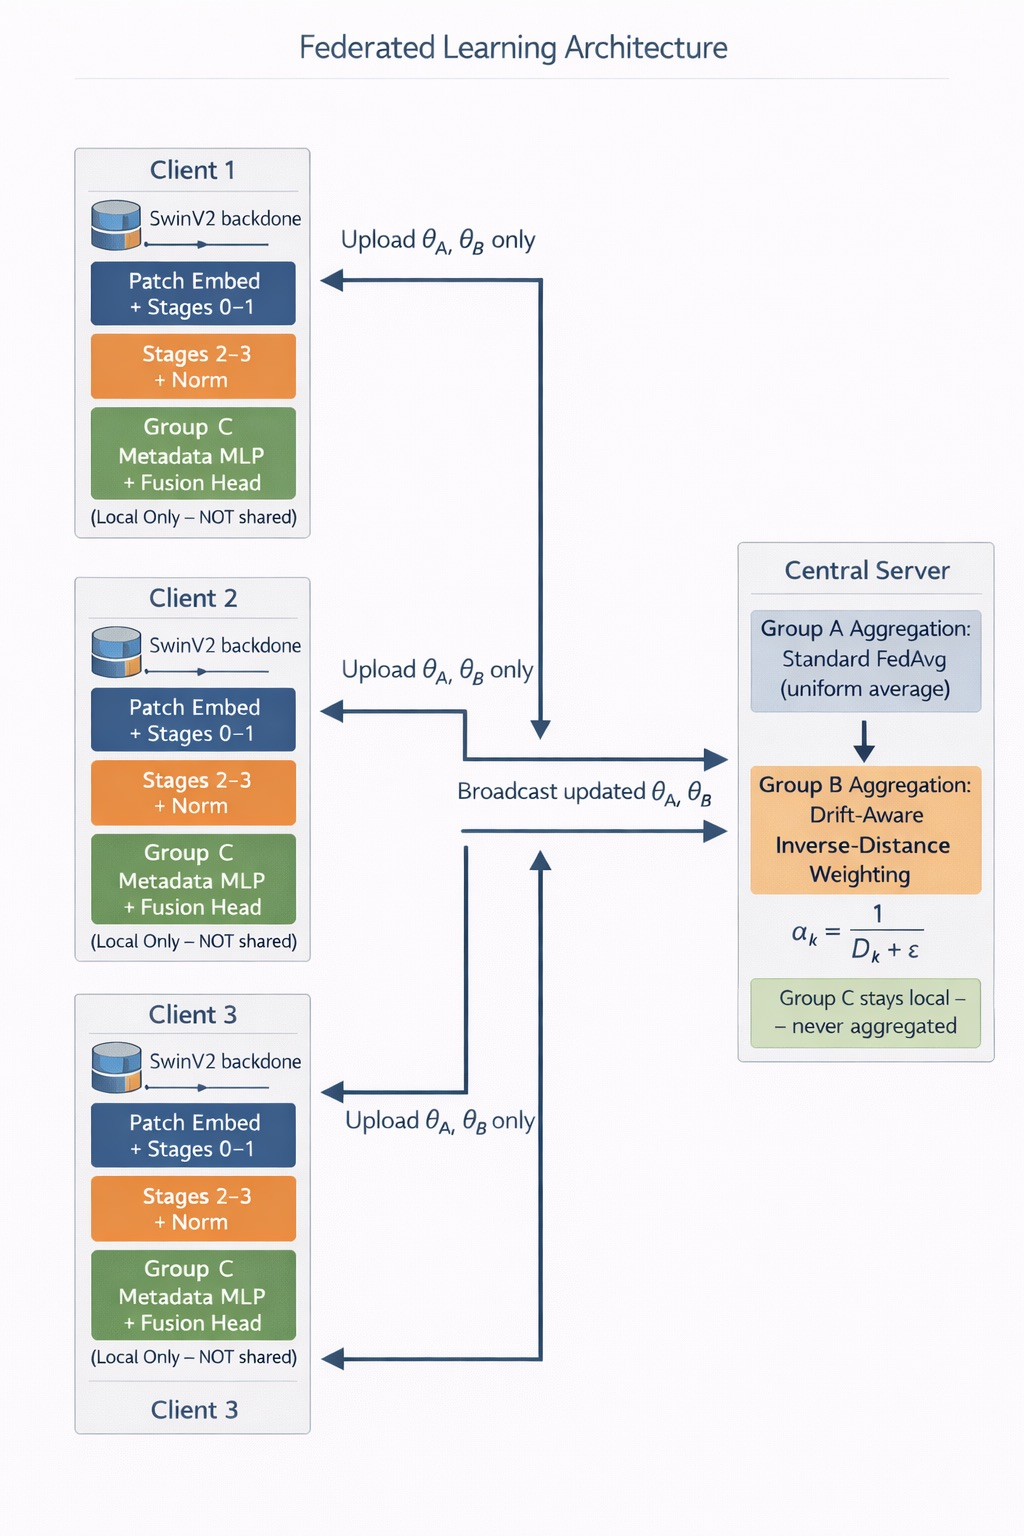
\includegraphics[width=0.90\truecolumnwidth]{images/federated learning.jpg}
\caption{Structure-aware federated aggregation architecture.}
\label{fig:framework}
\end{figure}

\subsection{Step 1: Dirichlet Non-IID Data Partitioning}

Each client's data is sampled from a Dirichlet prior to simulate the true heterogeneity that exists across multiple clients:

\begin{equation}
\label{eq:dirichlet}
\pi_k \sim \text{Dir}(\alpha)
\end{equation}

where $\pi_k \in \Delta^{C-1}$ is the class-proportion vector for client $k$ and $\alpha > 0$ is the concentration parameter. A smaller value for $\alpha$ gives more skewed class distributions across clients, and a larger value for $\alpha$ provides more uniform class distributions across clients.

The fraction of class-$c$ samples at client $k$ is:

\begin{equation}
\label{eq:class_proportion}
p_{kc} = \frac{n_{kc}}{n_k}
\end{equation}

The variance of these proportions across multiple clients is given by:

\begin{equation}
\label{eq:dirichlet_variance}
\text{Var}(p_{kc}) =
\frac{\alpha (C\alpha - \alpha)}
{(C\alpha)^2 (C\alpha + 1)}
\end{equation}

As $\alpha \to 0$, the variance increases, which represents the degree to which distributions across multiple clients will diverge based on the value assigned to the alpha parameter, leading to client gradients diverging:

\begin{equation}
\label{eq:gradient_divergence}
\nabla F_k(\theta) \neq \nabla F_j(\theta), \quad k \neq j
\end{equation}

This gradient misalignment is the core challenge in the federated learning scenario.

\subsection{Step 2: Centralized Training Baseline}

The data of all clients must be pooled together in order to create a reference upper bound:

\begin{equation}
\label{eq:pooled_data}
\mathcal{D} = \bigcup_{k=1}^{K} \mathcal{D}_k
\end{equation}

Empirical risk minimization (ERM) is used as the central target:

\begin{equation}
\label{eq:centralized_objective}
F(\theta)
=
\frac{1}{N}
\sum_{k=1}^{K}
\sum_{i=1}^{n_k}
\ell(f_\theta(x_i^k,m_i^k), y_i^k)
\end{equation}

where $\ell(\cdot,\cdot)$ is the per-sample cross-entropy loss. The dynamics of the updates are given by:

\begin{equation}
\label{eq:centralized_update}
\theta^{t+1} = \theta^t - \eta \nabla F(\theta^t)
\end{equation}

where $\nabla F(\theta^t) = \frac{1}{N}\sum_{k}\sum_{i} \nabla \ell(f_\theta(x_i^k,m_i^k), y_i^k)$.

The model is trained for $E$ epochs using AdamW with a cosine learning rate schedule:

\begin{equation}
\label{eq:centralized_admw}
\theta^{E} = \text{AdamW}(\theta^0, \mathcal{D})
\end{equation}

In a centralized context, there is no client drift and therefore no communication overhead. As such, the performance of this model acts as a reference upper bound for all subsequent federated experiments.

\begin{figure}[htbp]
\centering
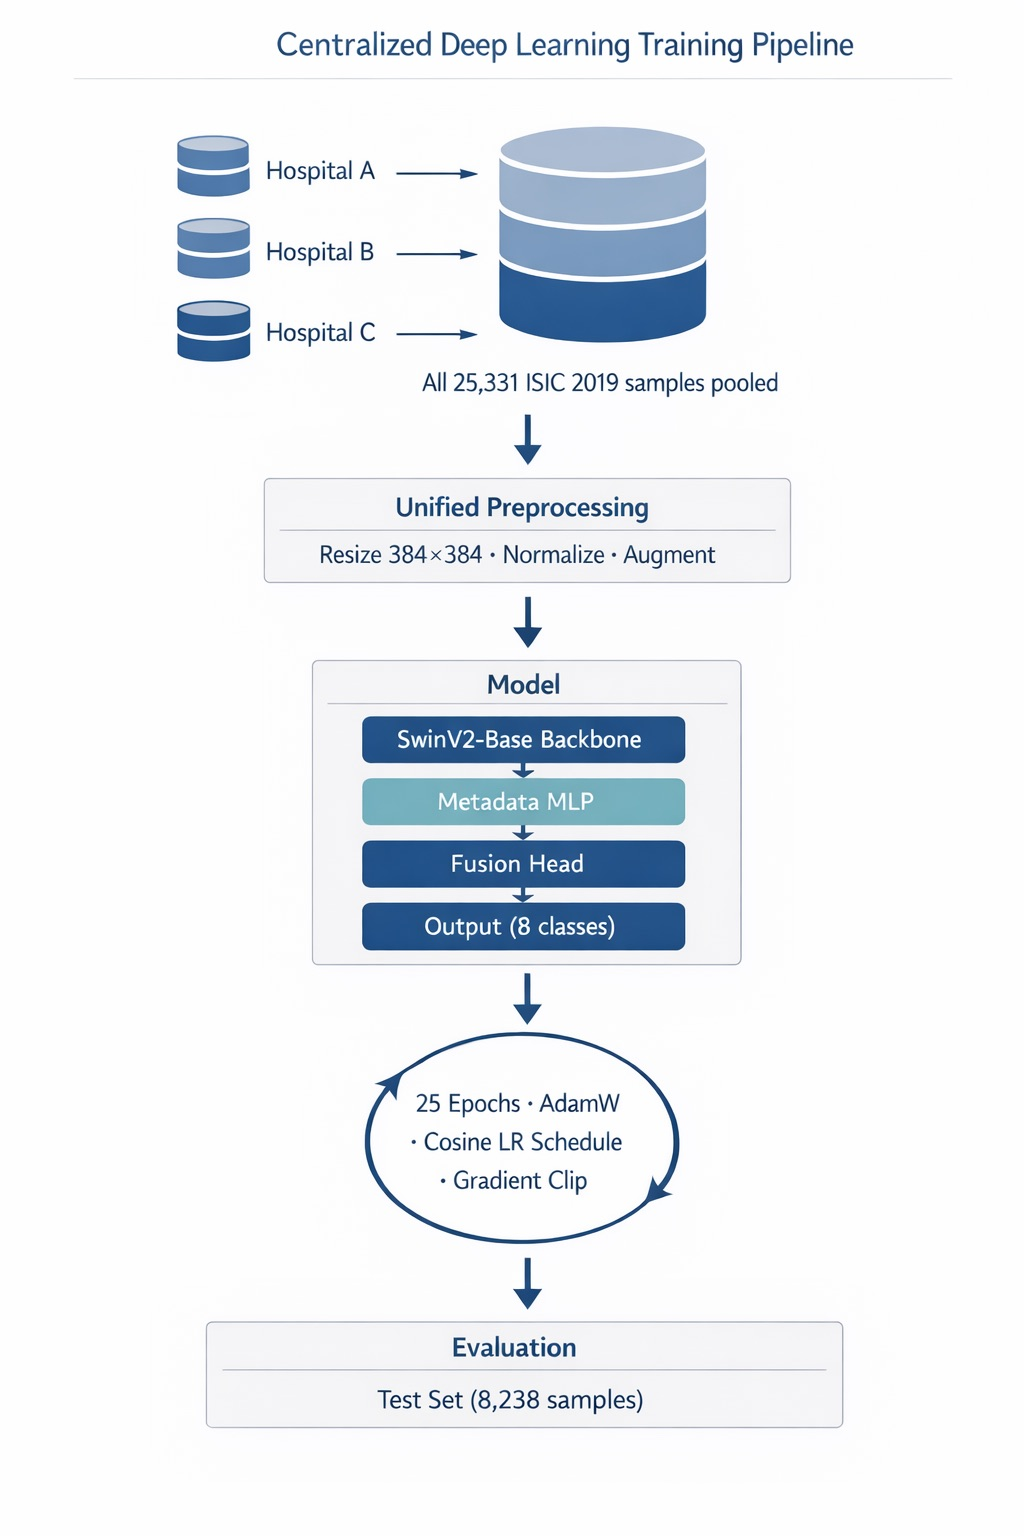
\includegraphics[width=0.45\textwidth]{images/centralized.jpg}
\caption{Centralized training pipeline using pooled multimodal data.}
\label{fig:centralized_flow}
\end{figure}

\subsection{Step 3: Federated Optimization Objective}

In federated learning, the global goal is the weighted average of all of the local objectives:

\begin{equation}
\label{eq:fed_objective}
F(\theta) = \sum_{k=1}^{K} \frac{n_k}{N} F_k(\theta)
\end{equation}

where $F_k(\theta)$ is the risk value for each client and is defined as:

\begin{equation}
\label{eq:local_risk}
F_k(\theta) = \frac{1}{n_k} \sum_{i=1}^{n_k} \ell(f_\theta(x_i^k,m_i^k), y_i^k)
\end{equation}

The server averages the gradients of all clients to generate the global gradient:

\begin{equation}
\label{eq:fed_gradient}
\nabla F(\theta) = \sum_{k=1}^{K} \frac{n_k}{N} \nabla F_k(\theta)
\end{equation}

When there are differences between the distributions of clients, this approximation becomes biased due to client drift.

\subsection{Step 4: Structure-Aware Parameter Decomposition}

To mitigate drift, \sadrift{} assigns each parameter to one of three functional groups:

\begin{equation}
\label{eq:param_decomp}
\theta = \{\theta_A, \theta_B, \theta_{C,k}\}
\end{equation}

\begin{itemize}
\item \textbf{Group A} ($\theta_A$) contains the patch embedding and early SwinV2 stages (0--1). These capture low-level visual features that generalize across institutions, and are aggregated by standard FedAvg.
\item \textbf{Group B} ($\theta_B$) contains the late SwinV2 stages (2--3) and layer normalization. These encode high-level semantics that are most sensitive to distribution shifts, and are aggregated with drift-aware weighting.
\item \textbf{Group C} ($\theta_{C,k}$) contains the client-specific metadata MLP and fusion head. These are never transmitted to the server.
\end{itemize}

The predicted output for sample $i$ at client $k$ is:

\begin{equation}
\label{eq:prediction}
\hat{y}_i^k = g_{\theta_{C,k}}\!\left(h_{\theta_A,\theta_B}(x_i^k),\, m_i^k\right)
\end{equation}

where $h_{\theta_A,\theta_B}$ is the shared SwinV2 backbone and $g_{\theta_{C,k}}$ is the local fusion head. As long as Group C is maintained locally, this enables the models to be personalized for each institution while still securing the confidentiality of the metadata.

\subsection{Step 5: Local Client Optimization}

Clients apply local training of the models via AdamW, where the backbone is trained at a $0.1\eta$ learning rate and the metadata MLP and fusion head use the $\eta$ learning rate. In addition, a cosine schedule with linear warmup is used for all parameters in both groups. The update rule is:

\begin{equation}
\label{eq:local_update}
\theta_k^{t+1} = \text{AdamW}(\theta^t, \nabla F_k(\theta^t), \eta)
\end{equation}

For the structured (grouped) parameters:

\begin{equation}
\label{eq:groupA_update}
\theta_{A,k}^{t+1} = \theta_A^t - \eta \nabla_{\theta_A} F_k
\end{equation}

\begin{equation}
\label{eq:groupB_update}
\theta_{B,k}^{t+1} = \theta_B^t - \eta \nabla_{\theta_B} F_k
\end{equation}

where $\nabla_{\theta_A} F_k$ and $\nabla_{\theta_B} F_k$ are the partial gradients of local risk at the clients. These per-client updates diverge across institutions under non-IID conditions. It is for this reason that drift-aware aggregation is needed, as described in Section~\ref{sec:drift_agg}.

\subsection{Step 6: Server-Side Drift-Aware Aggregation}
\label{sec:drift_agg}

Once local training is complete, the parameters for Groups A and B are uploaded to the server, where standard FedAvg is used to aggregate Group A and drift-aware weighting is used to de-emphasise updates from clients in Group B that deviate from the consensus. Furthermore, there are no changes to the local training objectives or the addition of hyperparameters.

\subsubsection{Distance Computation}

The server computes the mean across clients for every parameter tensor $l \in \theta_B$:

\begin{equation}
\label{eq:consensus_mean}
\bar{w}_l = \frac{1}{K} \sum_{k=1}^{K} w_{k,l}
\end{equation}

where $w_{k,l}$ is the tensor uploaded by client $k$. To calculate the client drift from the mean across clients, the Euclidean distance between the client update and the mean is computed:

\begin{equation}
\label{eq:drift_distance}
D_{k,l} = \| w_{k,l} - \bar{w}_l \|_2
\end{equation}

The $L_2$ norm is used here because model parameters exist within a Euclidean space. It is computationally efficient and gives an accurate measurement of how far every client update deviates from the mean across clients.

\subsubsection{Inverse-Distance Weighting}

Each client receives an unnormalised weight calculated using its drift:

\begin{equation}
\label{eq:inv_weight}
\alpha_{k,l} = \frac{1}{D_{k,l} + \epsilon}
\end{equation}

where $\epsilon = 10^{-6}$ avoids division by zero. This therefore gives more weight to clients that are near consensus and proportionally less weight to clients that are far from consensus.

The inverse approach is preferred to an exponential, e.g., $\exp(-\beta D_{k,l})$, as it has the following advantages:
\begin{itemize}
\item It does not require any additional sensitivity parameter $\beta$.
\item It will not cause a complete collapse of weights toward 0 in the case of large values of $D_{k,l}$.
\item A smooth heavy-tailed profile of decay in the weights is achieved.
\end{itemize}

Weights are normalized so that they sum to 1:

\begin{equation}
\label{eq:norm_weight}
\hat{\alpha}_{k,l} = \frac{\alpha_{k,l}}{\sum_{j=1}^{K} \alpha_{j,l}}
\end{equation}

The total combined Group B tensor is:

\begin{equation}
\label{eq:groupB_agg}
\theta_{B,l}^{t+1} = \sum_{k=1}^{K} \hat{\alpha}_{k,l} \cdot w_{k,l}
\end{equation}

\subsubsection{Convergence Analysis (Informal Argument)}

\noindent\textbf{Assumptions.}
The following informal argument assumes that each local objective $F_k$ is $L$-smooth (i.e., $\|\nabla F_k(\mathbf{u}) - \nabla F_k(\mathbf{v})\| \le L\|\mathbf{u}-\mathbf{v}\|$ for all $\mathbf{u},\mathbf{v}$) and that stochastic gradient noise has bounded second moment. This analysis is not a formal convergence proof and does not derive a rate; its purpose is to make precise the intuitive stability benefit of drift-aware attenuation under standard conditions.

Let $\Delta_k^t = \mathbf{w}_k^t - \mathbf{w}^t$ denote the local update of client $k$ at round $t$. Standard FedAvg combines updates as:

\begin{equation}
\label{eq:fedavg_agg}
\mathbf{w}^{t+1} = \mathbf{w}^t + \sum_{k=1}^{K} p_k \Delta_k^t
\end{equation}

where $p_k = n_k / N$. In \sadrift{}, each Group~B update is attenuated by a scalar factor $\gamma_k^t \in (0,1]$ derived from the inverse-distance weight $\hat{\alpha}_{k,l}$, giving an effective update $\tilde{\Delta}_k^t = \gamma_k^t \Delta_k^t$:

\begin{equation}
\label{eq:sadrift_agg}
\mathbf{w}^{t+1} = \mathbf{w}^t + \sum_{k=1}^{K} p_k \tilde{\Delta}_k^t
\end{equation}

Since $\gamma_k^t \le 1$ for all $k$, the $\ell_2$ norm of the aggregate step is bounded:

\begin{equation}
\label{eq:stability_bound}
\left\|\sum_{k=1}^K p_k \tilde{\Delta}_k^t\right\|_2
\;\le\;
\left\|\sum_{k=1}^K p_k \Delta_k^t\right\|_2
\end{equation}

That is, \sadrift{} never amplifies the aggregate update beyond what FedAvg would produce. Clients with the largest drift (large $D_{k,l}$, hence small $\gamma_k^t$) receive the smallest weight, pulling the aggregate toward the cross-client consensus.

Applying the standard descent lemma for $L$-smooth objectives and taking expectations over the stochastic gradient noise:

\begin{equation}
\label{eq:convergence}
\mathbb{E}[F(\mathbf{w}^{t+1})]
\;\le\;
F(\mathbf{w}^t)
- \eta \|\nabla F(\mathbf{w}^t)\|^2
+ \frac{\eta^2 L}{2}\,\mathbb{E}\!\left\|\sum_k p_k \tilde{\Delta}_k^t\right\|^2
\end{equation}

The third term—the noise amplification from the aggregate step—is bounded above by the corresponding FedAvg quantity via Eq.~\eqref{eq:stability_bound}. Intuitively, by suppressing drifted updates, \sadrift{} reduces the round-to-round oscillation of the global model without altering local training objectives. Deriving tight convergence rates under non-IID data and formally bounding gradient divergence under this aggregation scheme are left to future theoretical analysis.

\subsection{Step 7: End-to-End Federated Training Process}

Algorithm~\ref{alg:centralized} shows the centralized baseline. Algorithm~\ref{alg:federated} shows the full \sadrift{} federated procedure across $T$ communication rounds.

% ---- Algorithm 1: Centralized Training -------------------------------- %
\begin{algorithm}[t]
\caption{Centralized Training Baseline}
\label{alg:centralized}
\begin{algorithmic}[1]
\REQUIRE Dataset $\mathcal{D} = \bigcup_{k=1}^{K} \mathcal{D}_k$, pretrained backbone weights $\theta_A^0, \theta_B^0$, total epochs $E$, learning rate $\eta$
\ENSURE Trained model parameters $\theta^E$
\STATE Initialize model: $\theta^0 \leftarrow \{\theta_A^0,\, \theta_B^0,\, \theta_C^0\}$
\FOR{epoch $e = 1$ to $E$}
    \FOR{each mini-batch $(x_i, m_i, y_i) \in \mathcal{D}$}
        \STATE Compute logits: $\hat{y}_i = f_\theta(x_i, m_i)$
        \STATE Compute class-weighted CE loss with label smoothing:
               \[ \mathcal{L} = \mathcal{L}_{CE}^{\text{weighted}}(\hat{y}_i,\, y_i) \]
        \STATE Update via AdamW with cosine LR schedule:
               \[ \theta \leftarrow \theta - \eta\,\nabla_\theta\,\mathcal{L} \]
    \ENDFOR
    \STATE Evaluate on test set; record Balanced Accuracy, F1, ROC-AUC
\ENDFOR
\RETURN $\theta^E$
\end{algorithmic}
\end{algorithm}

% ---- Algorithm 2: FedSA-Drift Federated Training ---------------------- %
\begin{algorithm}[t]
\caption{\sadrift{}: Structure-Aware Drift-Regularized Federated Training}
\label{alg:federated}
\begin{algorithmic}[1]
\REQUIRE $K$ clients with local datasets $\{\mathcal{D}_k\}_{k=1}^K$, rounds $T$, local epochs $E$, learning rate $\eta$, $\epsilon = 10^{-6}$
\ENSURE Global shared parameters $\theta_A^T,\, \theta_B^T$; local parameters $\{\theta_{C,k}^T\}$
\STATE \textbf{Server:} Initialize $\theta_A^0,\, \theta_B^0$ from pretrained SwinV2-Base
\STATE Each client $k$ initializes local head $\theta_{C,k}^0$ independently
\FOR{round $t = 1$ to $T$}
    \STATE \textbf{Server} broadcasts $\theta_A^t,\, \theta_B^t$ to all $K$ clients
    \FOR{each client $k = 1$ to $K$ \textbf{(in parallel)}}
        \STATE Load received backbone: $\theta_{A,k} \leftarrow \theta_A^t$,\; $\theta_{B,k} \leftarrow \theta_B^t$
        \FOR{local epoch $e = 1$ to $E$}
            \FOR{each mini-batch $(x_i^k, m_i^k, y_i^k) \in \mathcal{D}_k$}
                \STATE $\hat{y}_i^k = g_{\theta_{C,k}}\!\left(h_{\theta_{A,k},\theta_{B,k}}(x_i^k),\, m_i^k\right)$
                \STATE $\mathcal{L}_k = \mathcal{L}_{CE}^{\text{weighted}}(\hat{y}_i^k,\, y_i^k)$
                \STATE Update all local params via AdamW (diff.\ LR):
                       $\theta_{A,k},\, \theta_{B,k},\, \theta_{C,k} \leftarrow \text{AdamW}(\mathcal{L}_k,\,\eta)$
            \ENDFOR
        \ENDFOR
        \STATE Upload $\theta_{A,k}^{t+1},\, \theta_{B,k}^{t+1}$ to server \quad \textit{(Group C stays local)}
    \ENDFOR
    \STATE \textbf{Server: Group A aggregation} (standard FedAvg):
           \[ \theta_A^{t+1} = \sum_{k=1}^{K} \frac{n_k}{N}\, \theta_{A,k}^{t+1} \]
    \STATE \textbf{Server: Group B drift-aware aggregation:}
    \FOR{each parameter tensor $l \in \theta_B$}
        \STATE Compute cross-client mean:
               $\bar{w}_l = \frac{1}{K}\sum_{k=1}^{K} w_{k,l}$
        \STATE Compute per-client drift:
               $D_{k,l} = \|w_{k,l} - \bar{w}_l\|_2$
        \STATE Compute inverse-drift weights:
               $\alpha_{k,l} = \frac{1}{D_{k,l} + \epsilon}$
        \STATE Normalize:
               $\hat{\alpha}_{k,l} = \alpha_{k,l} \big/ \sum_{j=1}^{K} \alpha_{j,l}$
        \STATE Aggregate:
               $\theta_{B,l}^{t+1} = \sum_{k=1}^{K} \hat{\alpha}_{k,l}\, w_{k,l}$
    \ENDFOR
    \STATE Evaluate global model $(\theta_A^{t+1}, \theta_B^{t+1})$ on test set
\ENDFOR
\RETURN $\theta_A^T,\, \theta_B^T,\; \{\theta_{C,k}^T\}_{k=1}^K$
\end{algorithmic}
\end{algorithm}

Compared to the centralized system (Algorithm~\ref{alg:centralized}), the federated implementation (Algorithm~\ref{alg:federated}) is structurally different. In centralized training, optimization runs directly on the pooled data, while in federated training, clients perform on-site training and the server enforces a global consensus over the shared backbone. The Group~C parameters that clients create using their on-site data are never sent to the server. This structure preserves the privacy of institutional metadata while still providing the capability for institutional specialisation.

\subsubsection{Training Flow Diagram}

Figure~\ref{fig:flow} illustrates one communication round of the training process.

\begin{figure}[t]
\centering
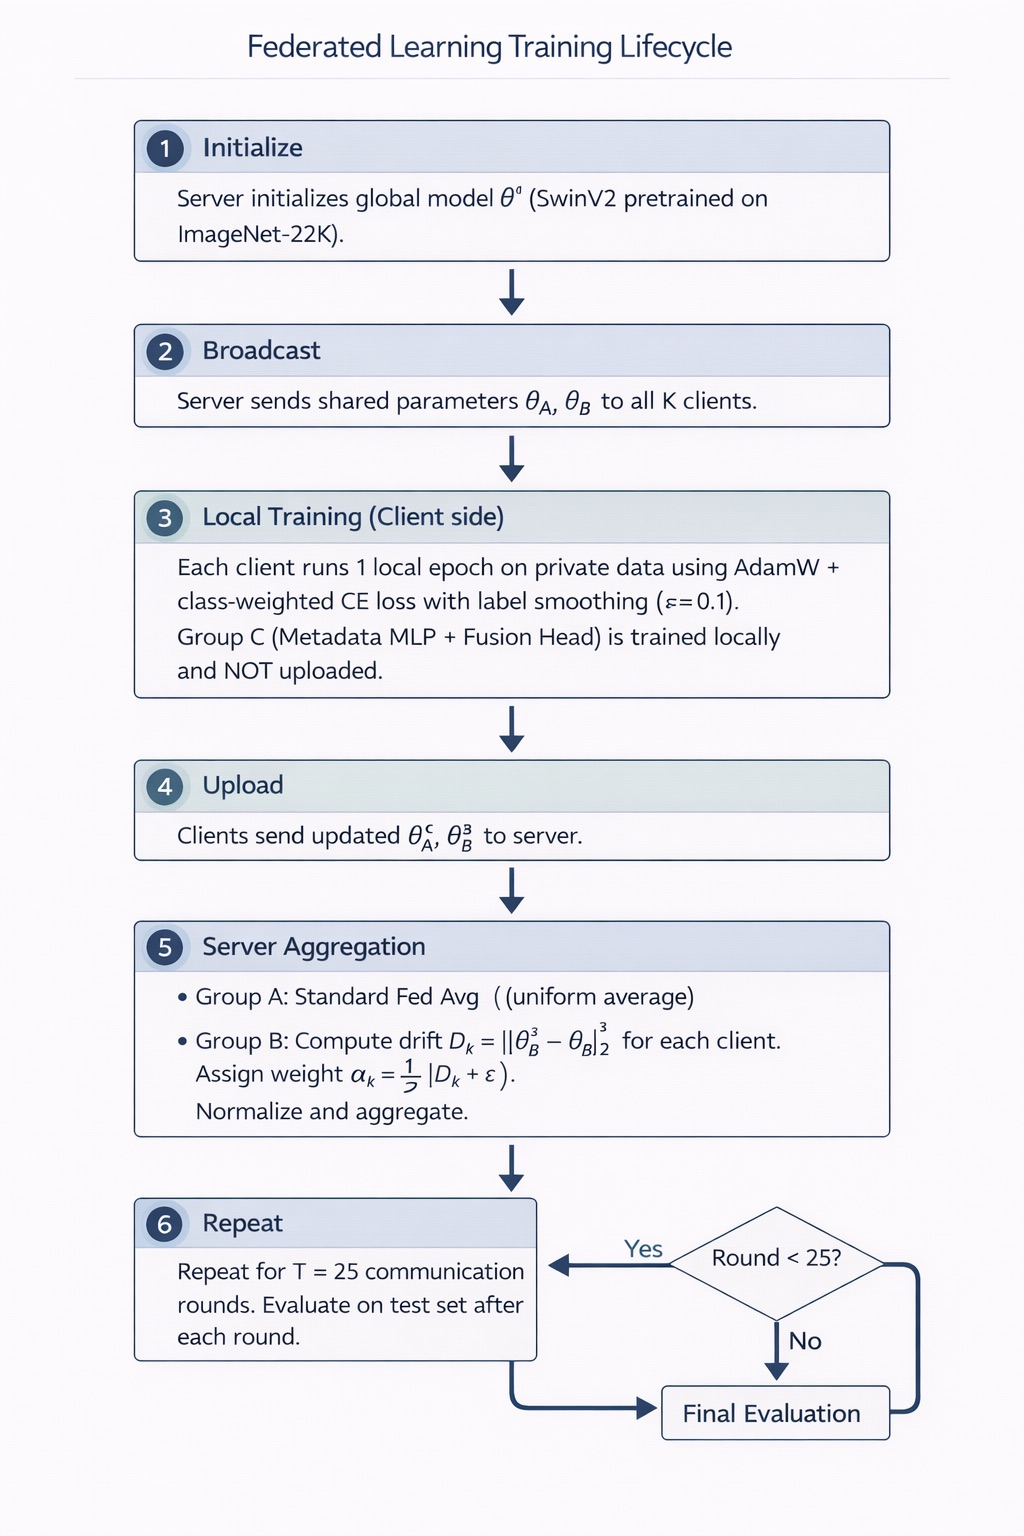
\includegraphics[width=0.72\truecolumnwidth]{images/flowing.jpg}
\caption{Federated training lifecycle across communication rounds.}
\label{fig:flow}
\end{figure}
% Experiments

\subsection{Dataset}

\sadrift{} is evaluated on the ISIC 2019 dataset, which consists of 25,331 dermoscopic images that encompass eight categories: Melanoma (MEL), Melanocytic Nevus (NV), Basal Cell Carcinoma (BCC), Actinic Keratosis (AK), Benign Keratosis (BKL), Dermatofibroma (DF), Vascular Lesion (VASC) and Squamous Cell Carcinoma (SCC). The unknown \texttt{UNK} class was removed before training. A separate test set of 8,238 images is available for final evaluation.

The images are resized to $384 \times 384$ pixels and normalised using ImageNet statistics ($\mu = [0.485, 0.456, 0.406]$, $\sigma = [0.229, 0.224, 0.225]$). The augmentation applied to the training images varies and includes random resized crops, random horizontal and vertical flips, rotations up to 45\textdegree, color jittering, RandAugment (2 ops, magnitude 9) and random erasing ($p=0.3$). All augmentations are applied during the training process only.

\subsection{Federated Data Partitioning}

The 25,331 training samples are randomly distributed across $K$ clients in accordance with a Dirichlet distribution centered at the concentration parameter $\alpha$. For instance, $\alpha = 1.0$ simulates near-IID conditions, while $\alpha = 0.5$ simulates moderately heterogeneous class distributions across clients. Each client is allocated a minimum of 2 class labels and at least 100 samples. If the partition does not pass these criteria, a new random seed is attempted, for a maximum of 50 times.

\subsection{Model Architecture}

The model architecture consists of a SwinV2-Base (\texttt{swinv2\_base\_window12to24\_192to384}, pre-trained on ImageNet-22K) backbone combined with a metadata branch. The SwinV2-Base implements shifted-window self-attention using 4 hierarchical levels to produce a 1024-dimensional feature representation from images. A two-layer metadata MLP ($13 \to 128 \to 128$ with GELU activation and dropout) provides a 128-dimensional feature representation of the age, sex, and anatomical site of each patient. This gives a total of 1152 dimensions as a concatenation of 1024 dimensions from the images and 128 dimensions from the metadata. The combined 1152-dimensional representation is then input to a fusion head that reduces the representation from $1152 \to 512 \to 8$ to classify each lesion into one of eight categories.

\subsection{Training Protocol}

Using centralized training, all 25,331 samples are used and no partitions are made with the data. Training occurs over 25 epochs. This serves as the upper bound of training performance.

Using federated training, FedAvg is used as the baseline aggregation method. The process for each communication round is as follows:
\begin{enumerate}
    \item The global model is broadcast from the server to all $K$ clients.
    \item Each client performs local training on its own data.
    \item Each client uploads the parameters to the server for both Group A and Group B.
    \item The server combines the updates and sends out a new global model.
\end{enumerate}
A total of 25 communication rounds are completed. The local training loss is computed using class-weighted cross-entropy with label smoothing ($\epsilon_s = 0.1$):

\begin{equation}
\label{eq:local_loss}
\mathcal{L}_k = \mathcal{L}_{CE}^{\text{weighted}}(f_{\theta}(x^k, m^k),\, y^k)
\end{equation}

Both drift correction and aggregation updates are completed only at the server; therefore, all local training objectives remain unchanged.

\subsection{Optimization Details}

The AdamW optimizer is configured via hyperparameters ($\beta_1=0.9$, $\beta_2=0.999$, weight decay $10^{-2}$) with differential learning rates. The SwinV2 backbone uses $0.1\eta$, while $\eta = 4 \times 10^{-4}$ is used for the metadata MLP and the fusion head. The learning rate schedule consists of a cosine decay following a linear warmup of 2 epochs. Gradient clipping is applied so that gradients remain at most 1.0.

Each class is weighted by the inverse of its class frequency. At every round, the \texttt{WeightedRandomSampler} oversamples the low-frequency classes at each client. A single batch size of 32 (16 per device with 2 gradient accumulation steps) is used during centralized training. The batch size is set to 16 with 1 local epoch per round at each federated client.

All experiments were completed using FP16 mixed precision on a single NVIDIA A40 GPU with 48~GB of RAM. All federated experiments were conducted via simulation on a single computing device.

\subsection{Evaluation Metrics}

The test set containing 8,238 samples is used for all evaluations. The following metrics are reported:
\begin{itemize}
    \item Top-1 Accuracy and Balanced Accuracy
    \item Macro F1-Score and Macro ROC-AUC
    \item Macro Average Precision
    \item Per-class classification report and confusion matrix
\end{itemize}

In addition to the above metrics, fairness evaluation is performed using:
\begin{itemize}
    \item Worst-case client accuracy (minimum across all clients)
    \item Inter-client standard deviation of accuracy
\end{itemize}

\section{Results and Discussion}

The performance of \sadrift{} is assessed along three dimensions: global classification accuracy, worst-client fairness and computational efficiency. Numerical comparisons with recent state-of-the-art methods are also provided.

\subsection{Centralized Upper Bound Performance}

\sadrift{} was trained in a centralized fashion on all 25,331 samples from ISIC 2019 for 25 epochs to obtain a peak Balanced Accuracy of \textbf{0.8867} at Epoch~21. Top-1 Accuracy at this point was 0.8566, Macro ROC-AUC was 0.9607 and Macro F1-score was 0.8237. Performance saturated after Epoch~21, demonstrating convergence. Training curves can be found in Figure~\ref{fig:centralized_curves}. The terminal output is also available in Figure~\ref{fig:cent_terminal}.

The performance of \sadrift{}'s centralized baseline exceeds that of the ISIC 2019 Challenge winner by \citet{Gessert2020}, who used heavily augmented multi-resolution EfficientNets combined with metadata to achieve a cross-validation Balanced Accuracy of $74.2 \pm 1.1\%$ and an official test accuracy of 63.6\%. \sadrift{}'s centralized baseline exceeds this value by \textbf{+14.47 percentage points}. Other state-of-the-art centralized hybrid methods, such as MedFusionNet~\citep{Naeem2025}, have been able to achieve 97.5--98.0\% raw accuracy; however, they cannot be deployed across hospital networks without contravening GDPR~\citep{Voigt2017} and HIPAA requirements.

\begin{figure*}[t]
\centering
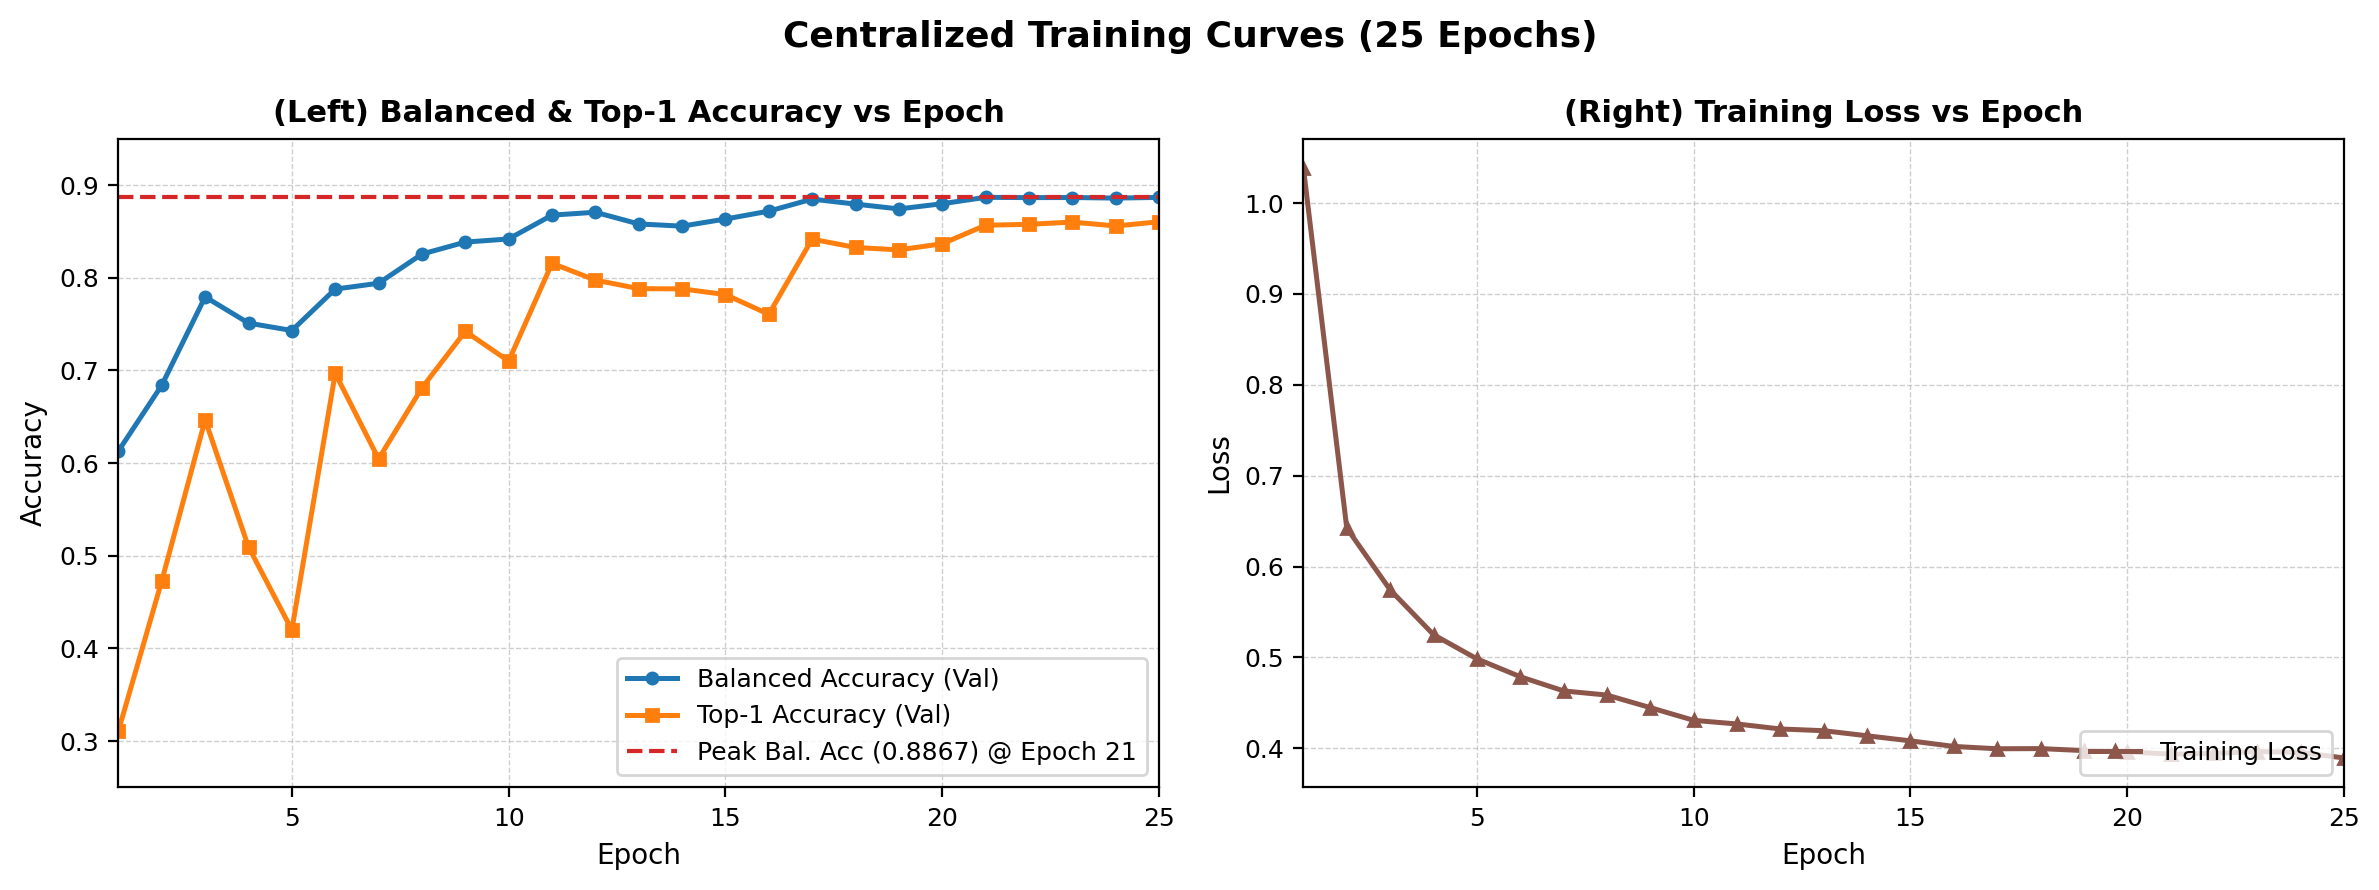
\includegraphics[width=\textwidth]{images/centralized_training_curves.png}
\caption{Centralized training curves over 25 epochs: (Left) Balanced Accuracy and Top-1 Accuracy; (Right) Training Loss. Peak Balanced Accuracy of 0.8867 is reached at Epoch~21.}
\label{fig:centralized_curves}
\end{figure*}

\begin{figure*}[t]
\centering
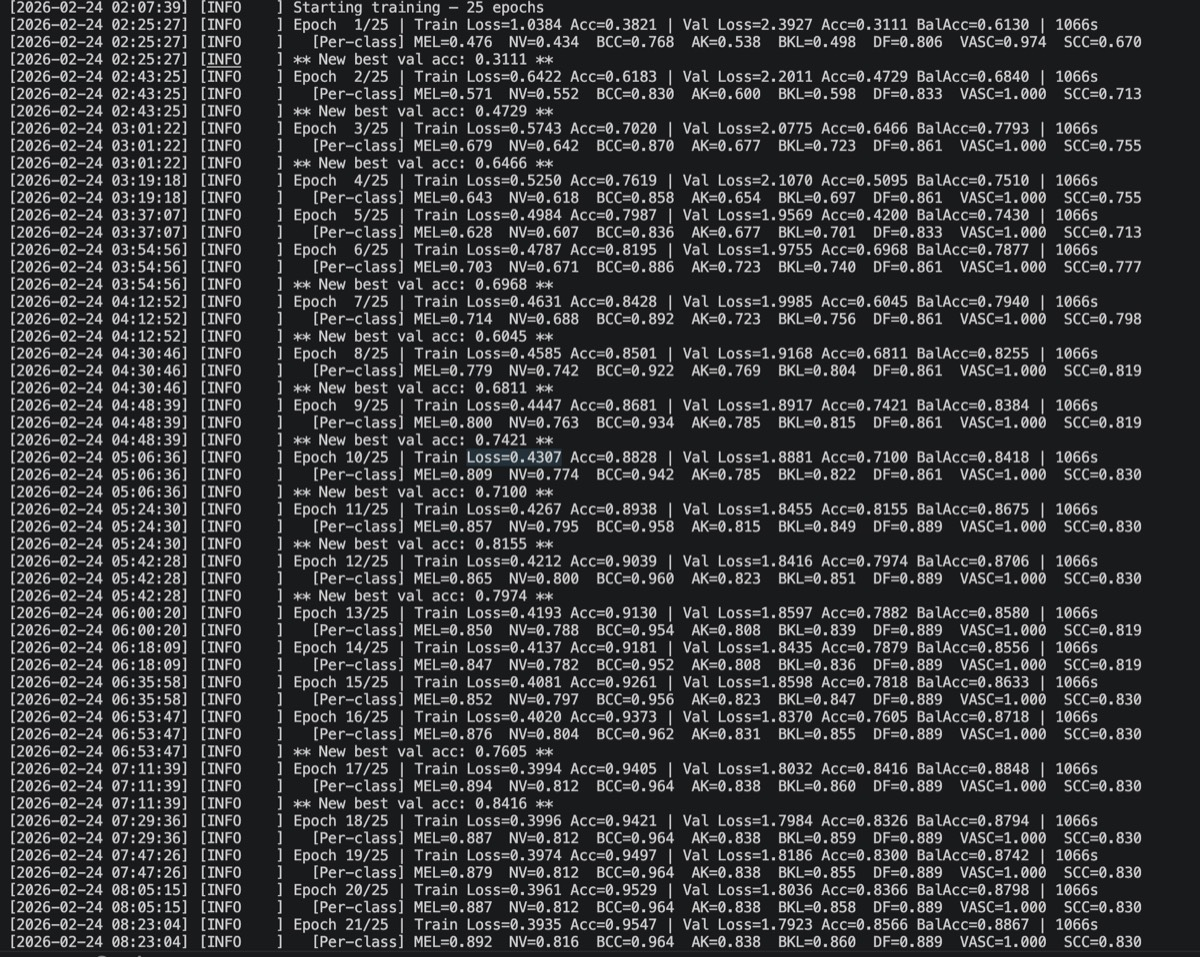
\includegraphics[width=0.80\textwidth]{images/centralized-run1.jpg}\\[4pt]
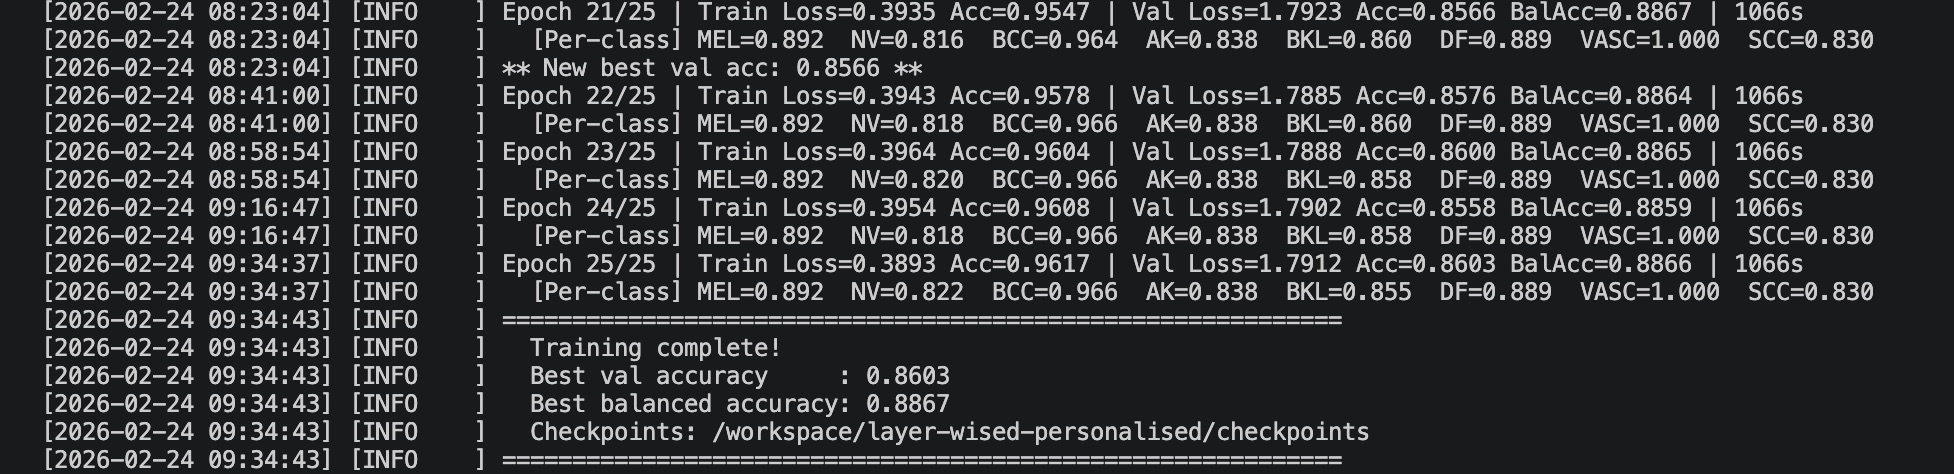
\includegraphics[width=0.80\textwidth]{images/centralized-run2.jpg}
\caption{Centralized training run terminal output (NVIDIA A40, RunPod): (Top) Epochs~1--13 showing progressive improvement in validation Balanced Accuracy; (Bottom) Epochs~14--25 converging to peak Balanced Accuracy of 0.8867 at Epoch~21, with per-class recall and final training summary.}
\label{fig:cent_terminal}
\end{figure*}

\subsection{Consolidated Federated Performance}

The results from each experimental configuration have been summarized in Table~\ref{tab:consolidated_performance}. These summary results consist of the centralized upper bound performance as well as that found from the two different levels of Dirichlet heterogeneity and the two aggregation methods used. All comparisons made after this step reference Table~\ref{tab:consolidated_performance}.

\begin{table*}[t]
\centering
\caption{Consolidated Performance of \sadrift{} Across All Experimental Configurations}
\label{tab:consolidated_performance}
\begin{tabular}{llccccc}
\toprule
Experiment & Config ($\alpha$, $K$) & Drift Strategy & Global Bal.\ Acc & Worst Client Acc & Std Dev (Acc) & Avg Round Time \\
\midrule
Centralized & N/A & N/A & 0.8867 & N/A & N/A & 1066\,s \\
Fed-2 (Baseline) & $\alpha{=}1.0$, $K{=}3$ & Uniform (Off) & \textbf{0.8314} & 0.6479 & 0.0182 & 1297\,s \\
Fed-1 (Ours) & $\alpha{=}1.0$, $K{=}3$ & Adaptive (On) & 0.8209 & \textbf{0.7850} & \textbf{0.0076} & 1301\,s \\
Fed-4 (Baseline) & $\alpha{=}0.5$, $K{=}5$ & Uniform (Off) & \textbf{0.7622} & 0.4800 & 0.0833 & 1439\,s \\
Fed-3 (Ours) & $\alpha{=}0.5$, $K{=}5$ & Adaptive (On) & 0.7066 & \textbf{0.5705} & \textbf{0.0511} & 1450\,s \\
\bottomrule
\end{tabular}
\end{table*}

\subsection{Mitigating Exacerbated Drift and Ensuring Client Fairness}

In multimodal federated networks that keep metadata heads local but share a common backbone, client drift can be exacerbated as the visual backbone is driven toward different local optima \citep{Zhu2025}. This paper confirms this through experiments with \sadrift{} and describes it in more detail below.

\subsubsection{Near-IID Setting ($\alpha = 1.0$, $K = 3$)}

With $K{=}3$ clients and $\alpha{=}1.0$, the class distributions are nearly uniform across clients. Two different aggregation methodologies are compared: 1) standard FedAvg, and 2) \sadrift{} that uses drift-aware weighting on Group~B.

Under these mild levels of client heterogeneity, FedAvg achieves a balanced global accuracy of 0.8314; however, the worst-performing client drops to 0.6479, which would not be apparent from the global average. Using \sadrift{}, the worst-client accuracy increases by \textbf{+13.71 points} to 0.7850, and the inter-client standard deviation decreases by \textbf{58\%} from 0.0182 to 0.0076 (observed in a single experimental trial). Both methods retain 93--94\% of centralized performance globally.

The round-by-round training curves and terminal outputs (Figures~\ref{fig:near_iid_sadrift_bundle} and~\ref{fig:near_iid_fedavg_bundle}) clearly demonstrate that the two methodologies converge toward the centralized upper bound, and that \sadrift{} achieves a tighter client accuracy band and a higher worst-client floor compared to FedAvg.

\begin{figure*}[!t]
\centering
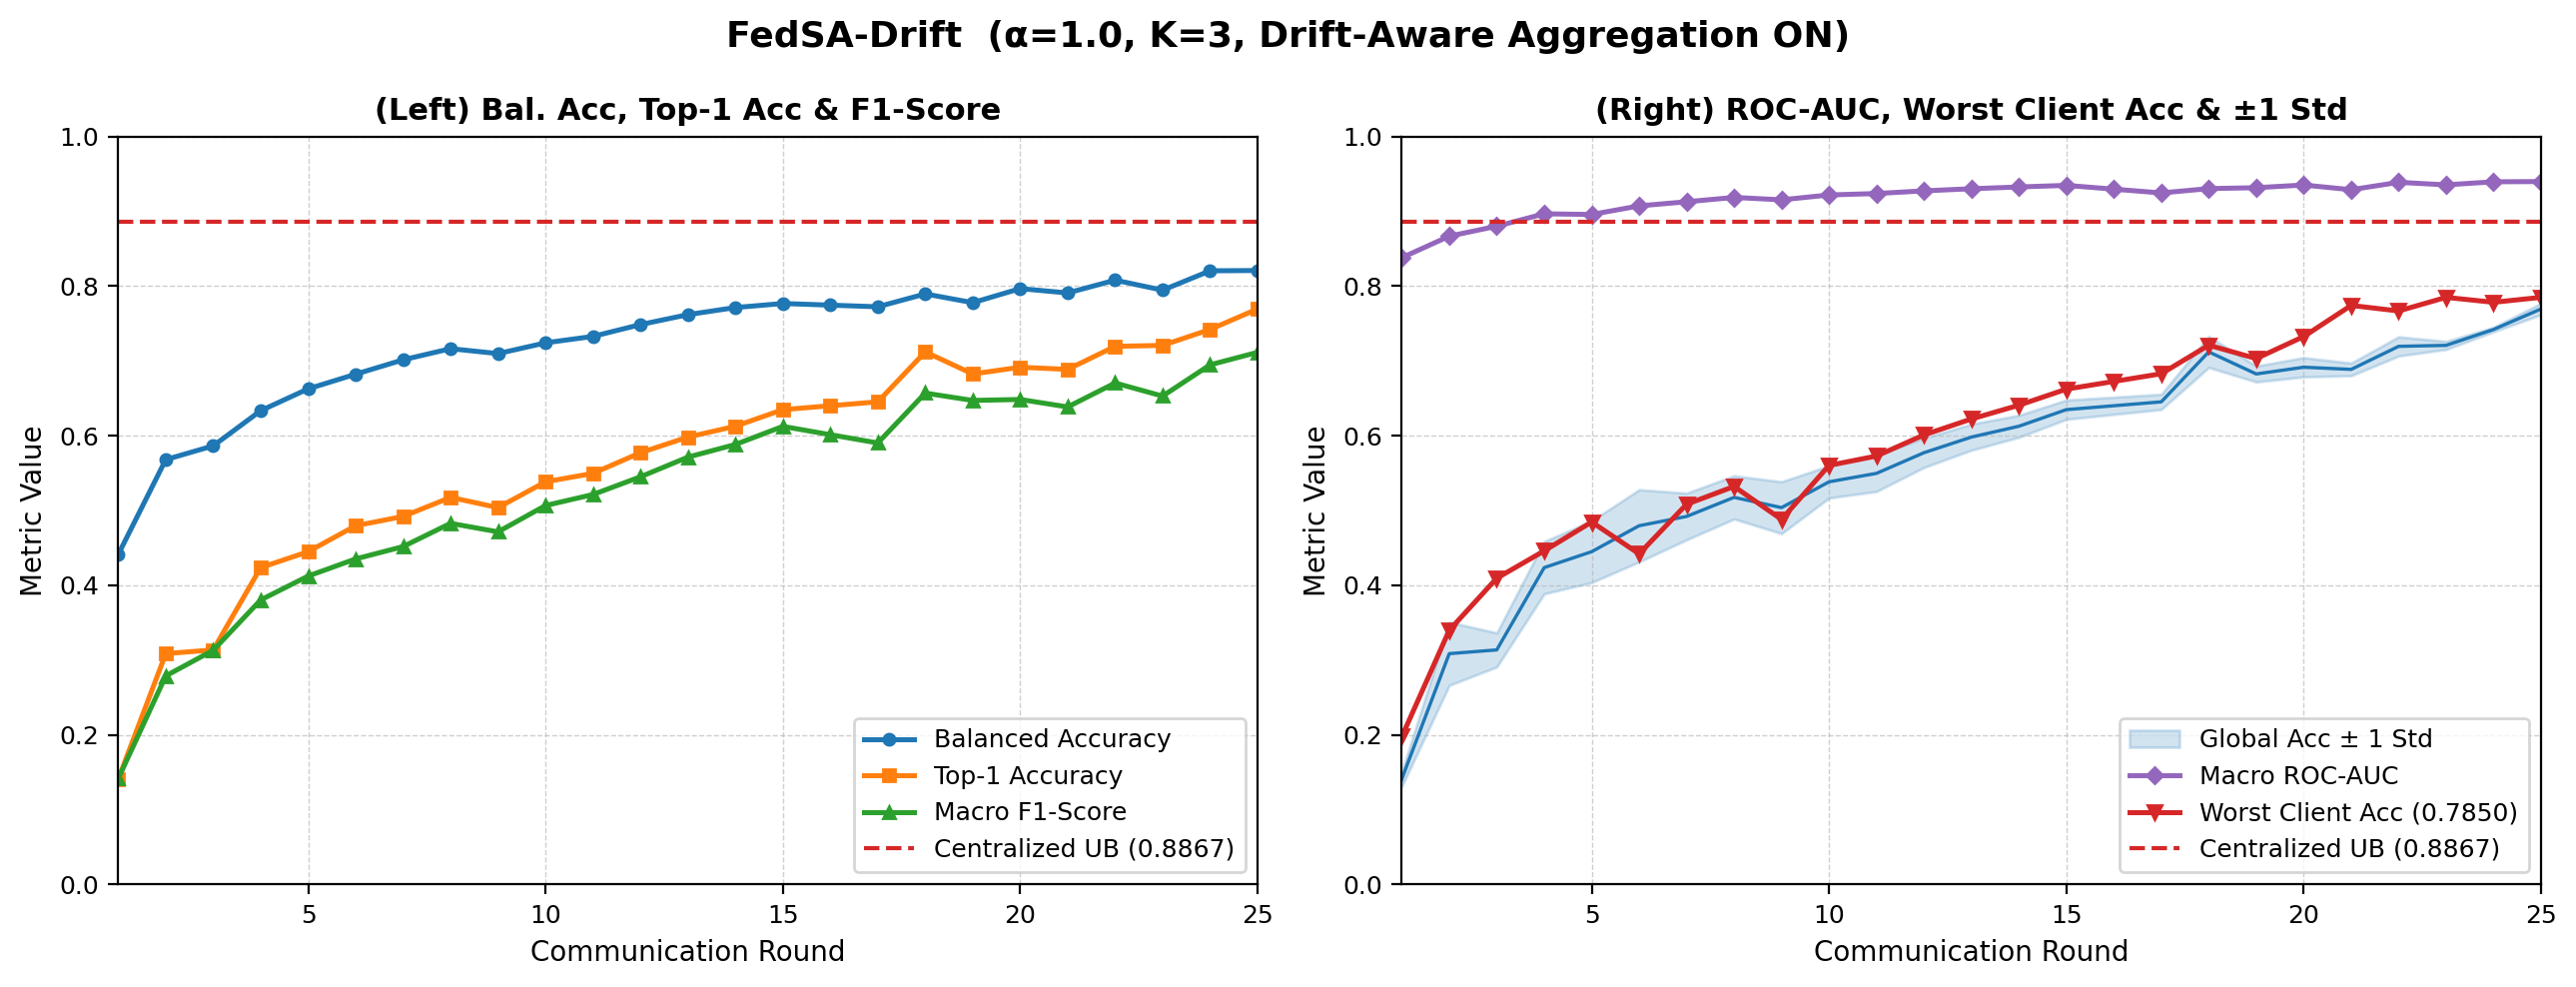
\includegraphics[width=0.80\textwidth]{images/sa_drift_near_iid_curves.png}\\[4pt]
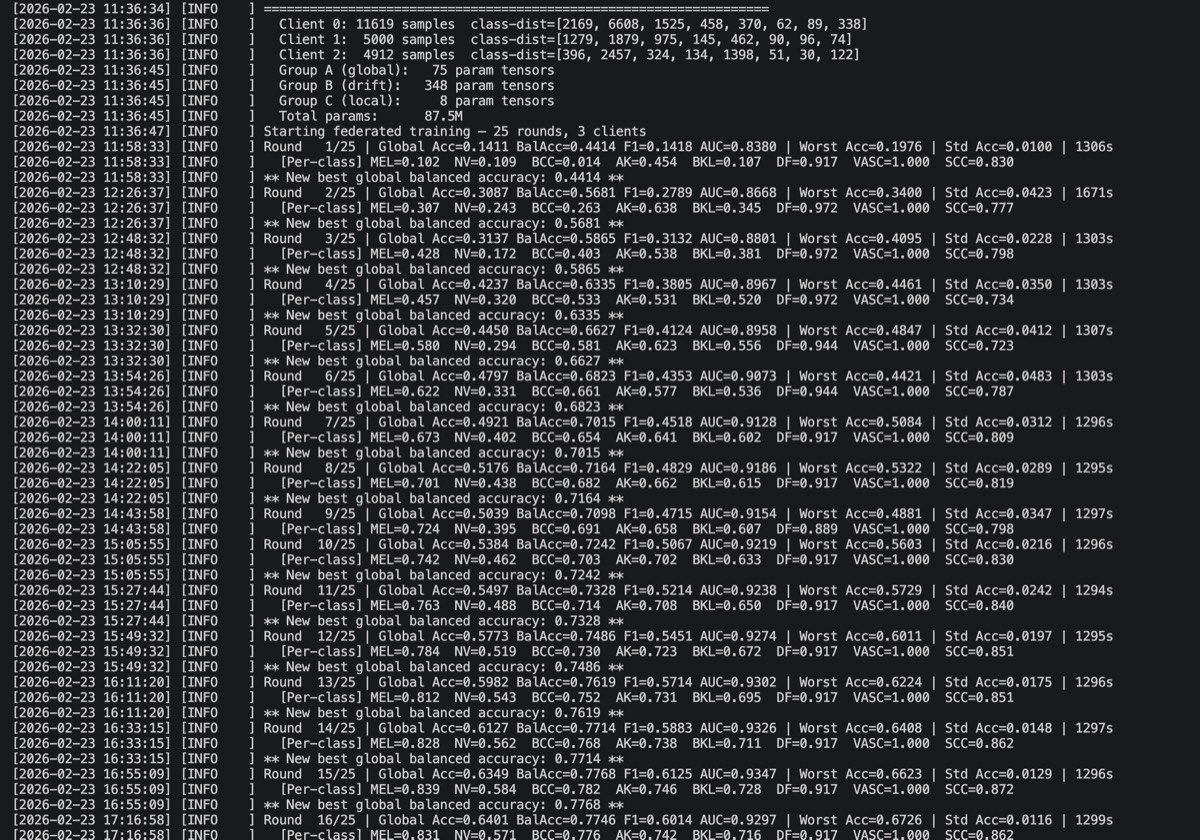
\includegraphics[width=0.80\textwidth]{images/a=1, client=3, drift= True1.jpg}\\[4pt]
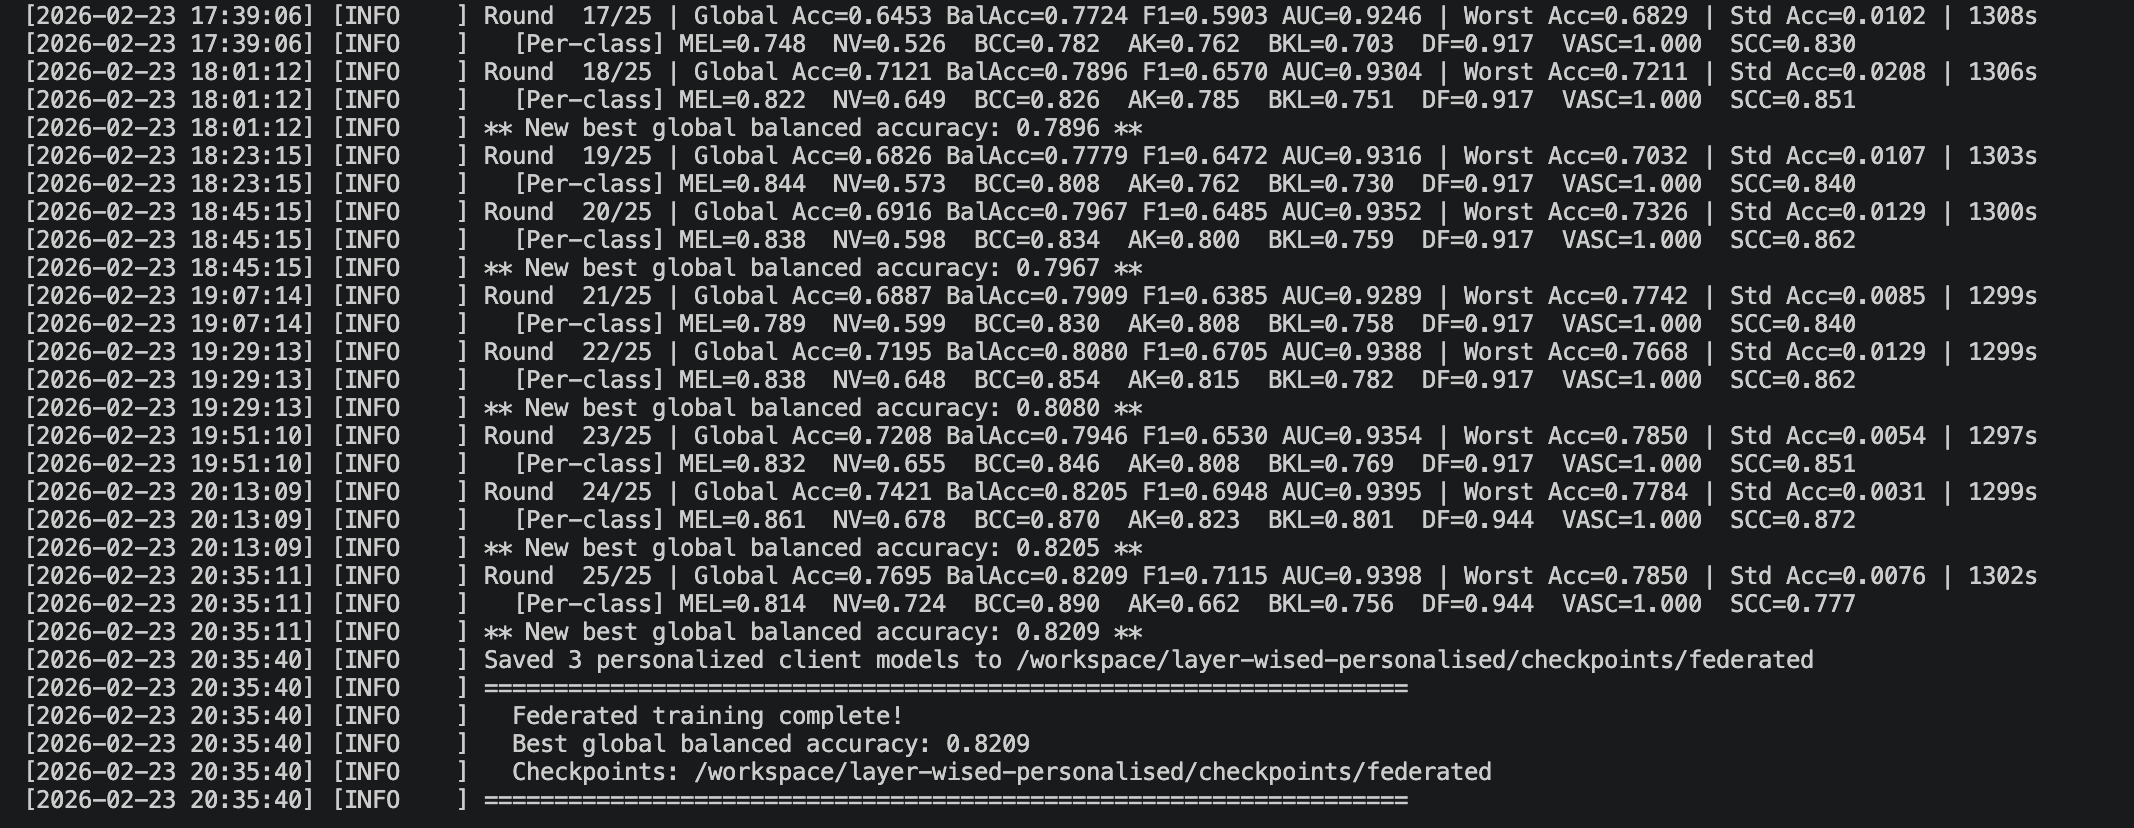
\includegraphics[width=0.80\textwidth]{images/a=1, client=3, drift= True2.png}
\caption[FedSA-Drift near-IID (alpha=1.0, K=3)]{FedSA-Drift near-IID setting ($\alpha{=}1.0$, $K{=}3$): top panel shows convergence metrics; middle and bottom panels show terminal outputs (Rounds 1--13 and 14--25). Final Balanced Accuracy: 0.8209, Worst Client Accuracy: 0.7850.}
\label{fig:near_iid_sadrift_bundle}
\end{figure*}

\begin{figure*}[!t]
\centering
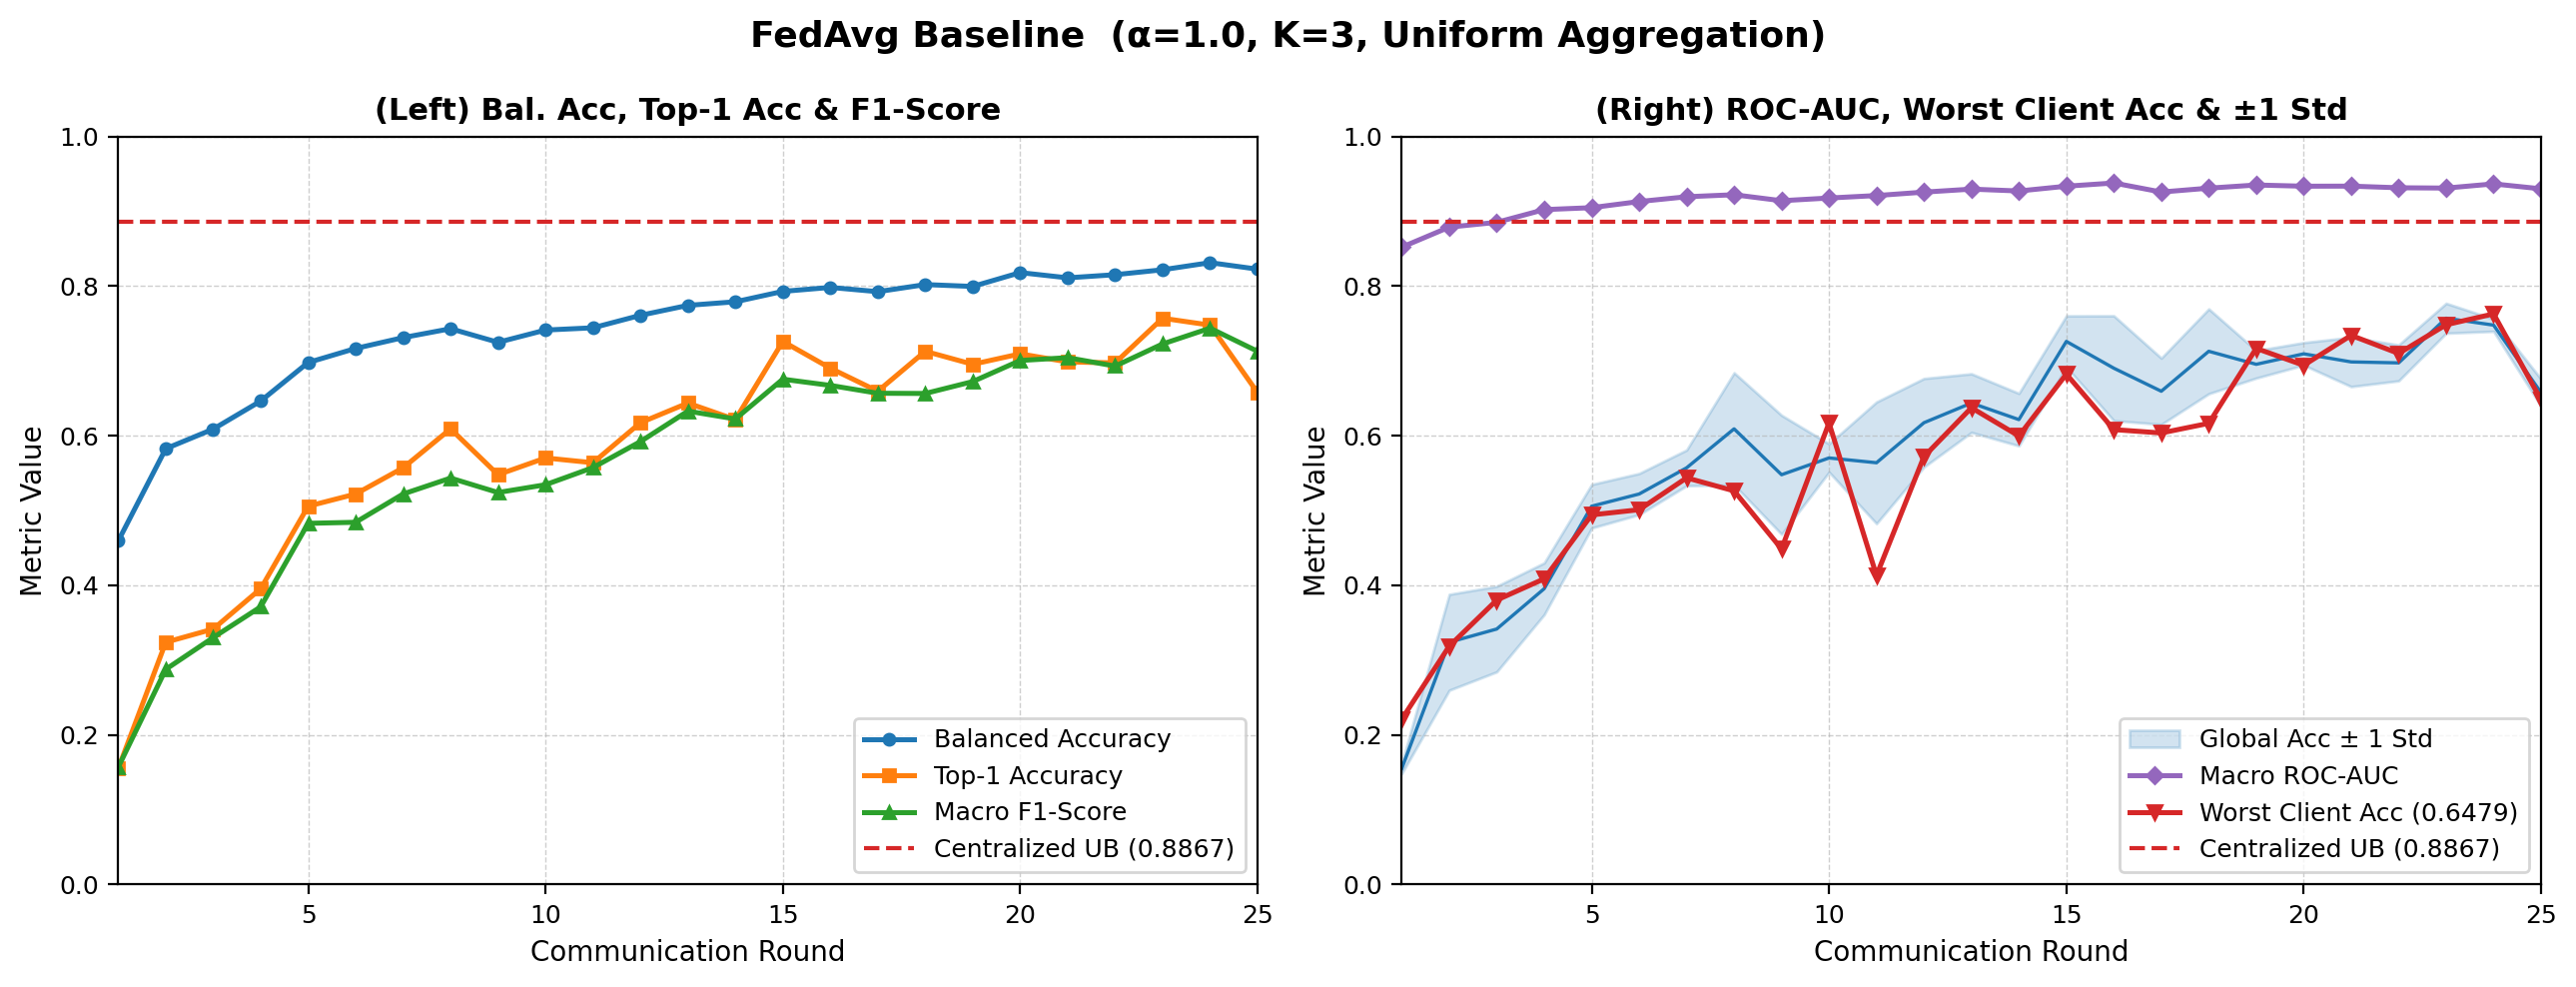
\includegraphics[width=0.80\textwidth]{images/fedavg_near_iid_curves.png}\\[4pt]
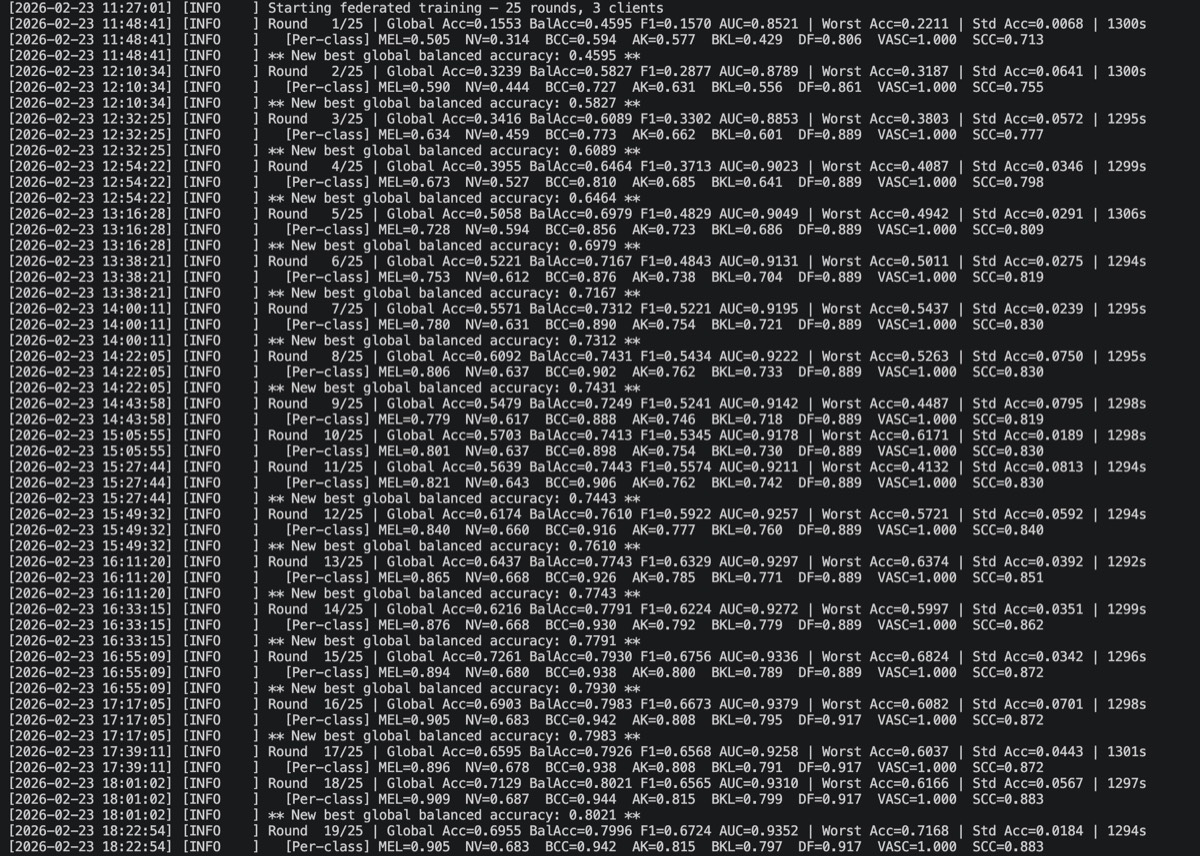
\includegraphics[width=0.80\textwidth]{images/a=1, client=3, drift= False1.jpg}\\[4pt]
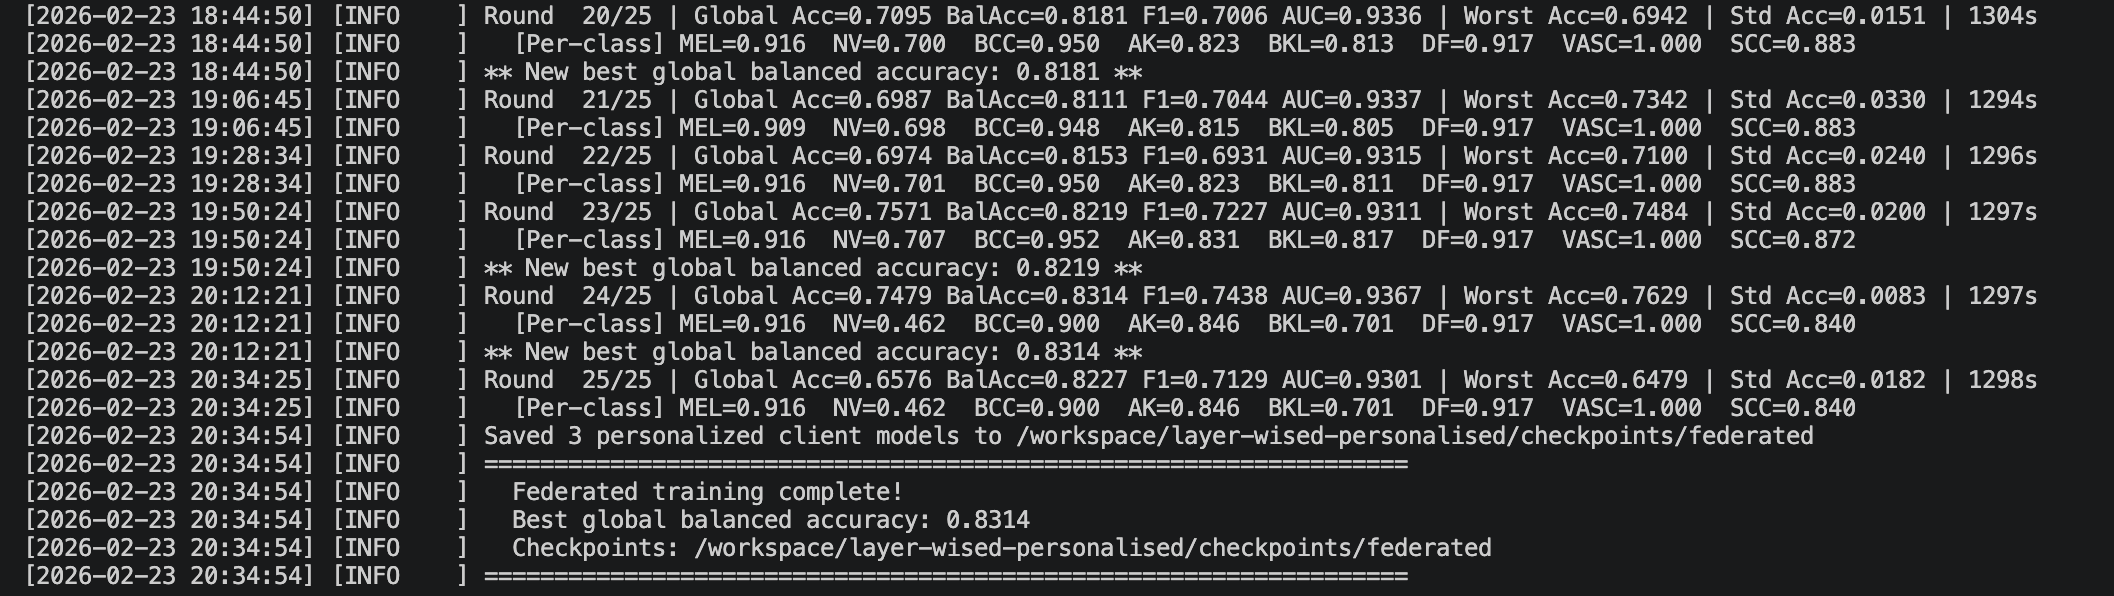
\includegraphics[width=0.80\textwidth]{images/a=1, client=3, drift= False2.png}
\caption[FedAvg near-IID (alpha=1.0, K=3)]{FedAvg near-IID setting ($\alpha{=}1.0$, $K{=}3$): top panel shows convergence metrics; middle and bottom panels show terminal outputs (Rounds 1--13 and 14--25). Final Balanced Accuracy: 0.8314, Worst Client Accuracy: 0.6479.}
\label{fig:near_iid_fedavg_bundle}
\end{figure*}

\subsubsection{Moderately Heterogeneous Setting ($\alpha = 0.5$, $K = 5$)}

The introduction of significant class imbalance across institutions ($K{=}5$ and $\alpha{=}0.5$) produces a more realistic clinical scenario. The use of \sadrift{} to correct for drift provides an improvement over the worst client (lowest accuracy) of \textbf{+9.05 percentage points} from 0.4800 to 0.5705 and reduces inter-client variance by \textbf{38.7\%} from 0.0833 to 0.0511 (observed in a single experimental trial). The results in Figures~\ref{fig:non_iid_sadrift_bundle} and~\ref{fig:non_iid_fedavg_bundle} indicate that the convergence of the different model types will be slower and noisier than in the near-IID case. Therefore, the improvement to the performance floor is clearly visible in this comparison.

\begin{figure*}[!t]
\centering
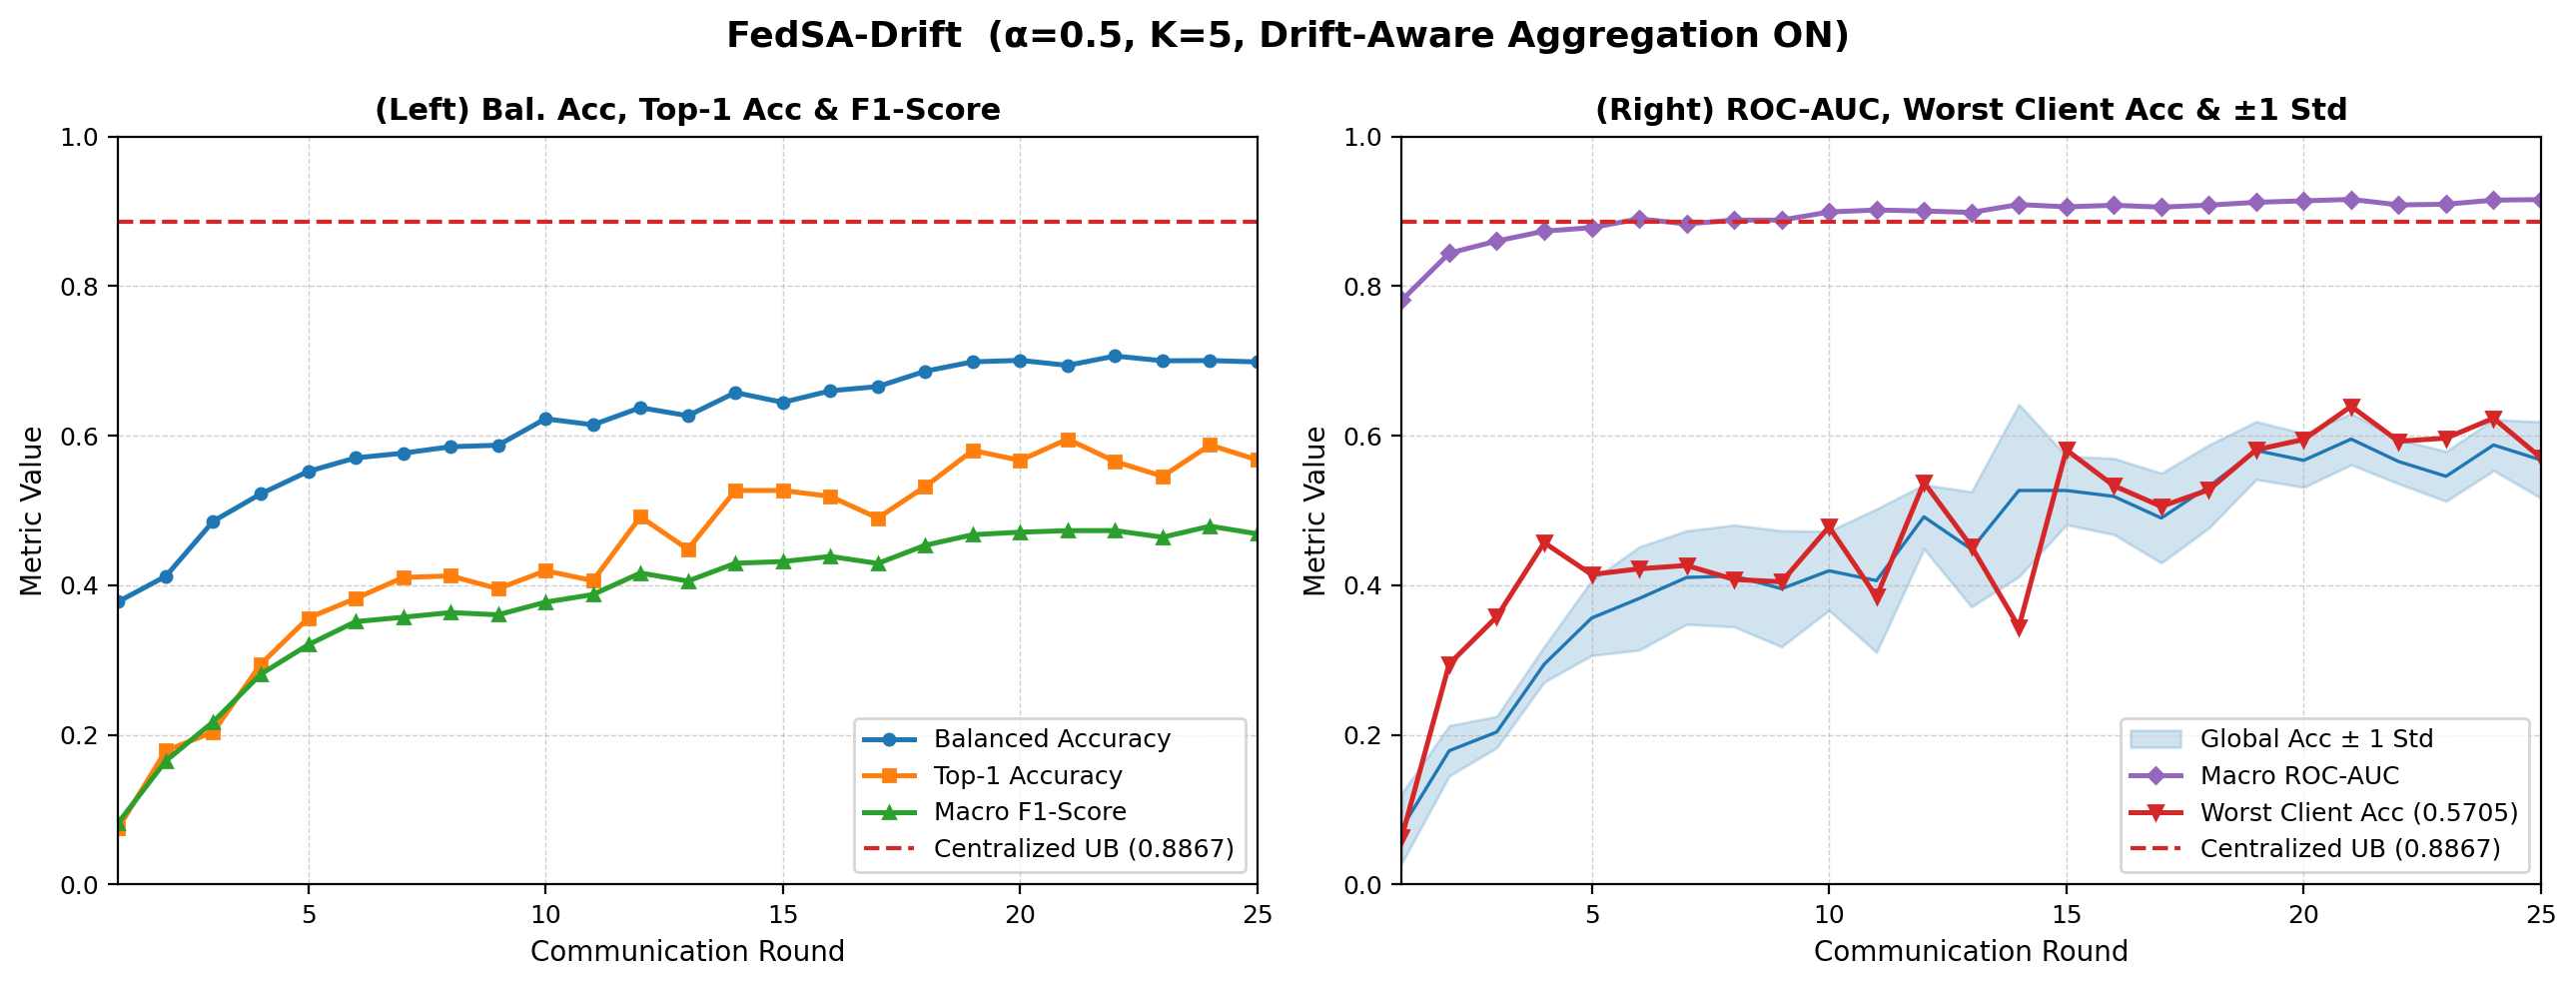
\includegraphics[width=0.80\textwidth]{images/sa_drift_non_iid_curves.png}\\[4pt]
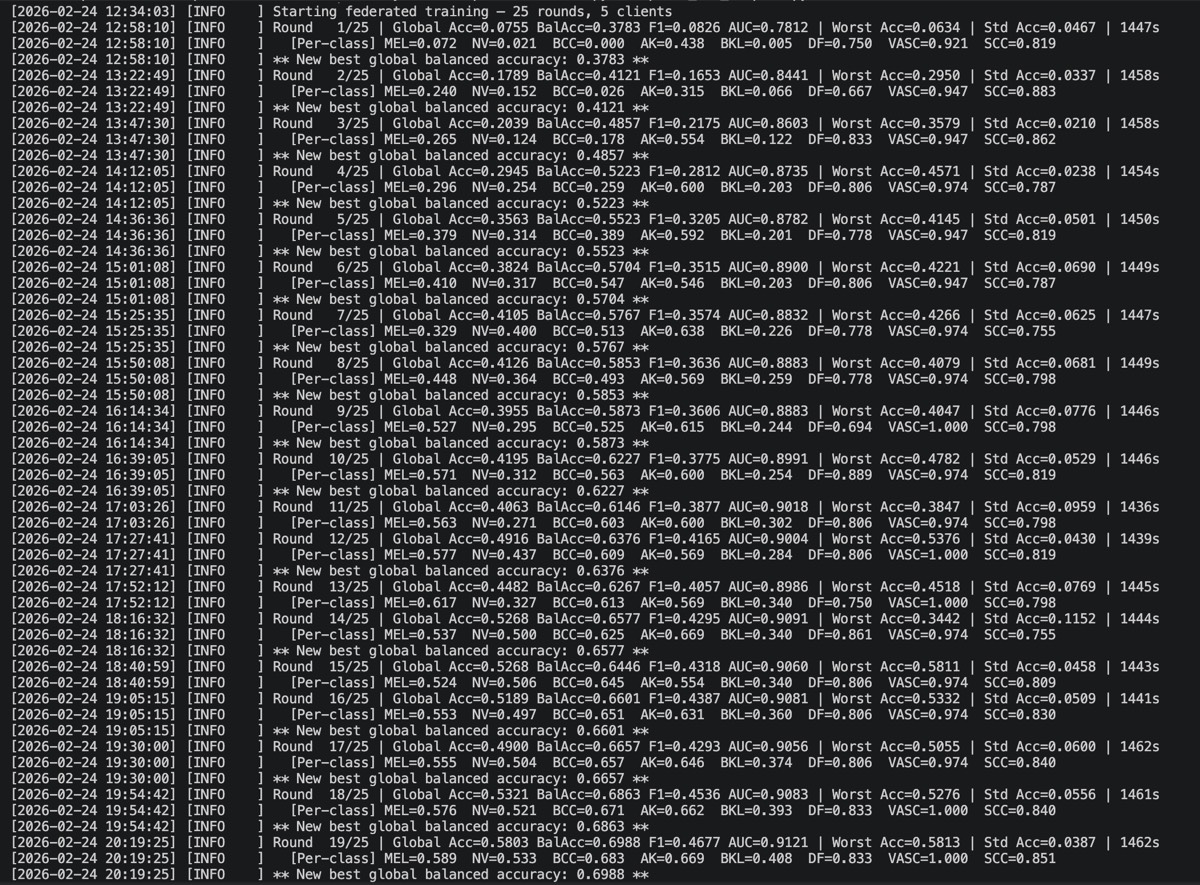
\includegraphics[width=0.80\textwidth]{images/a=0.5, client=5, drift= True1.jpg}\\[4pt]
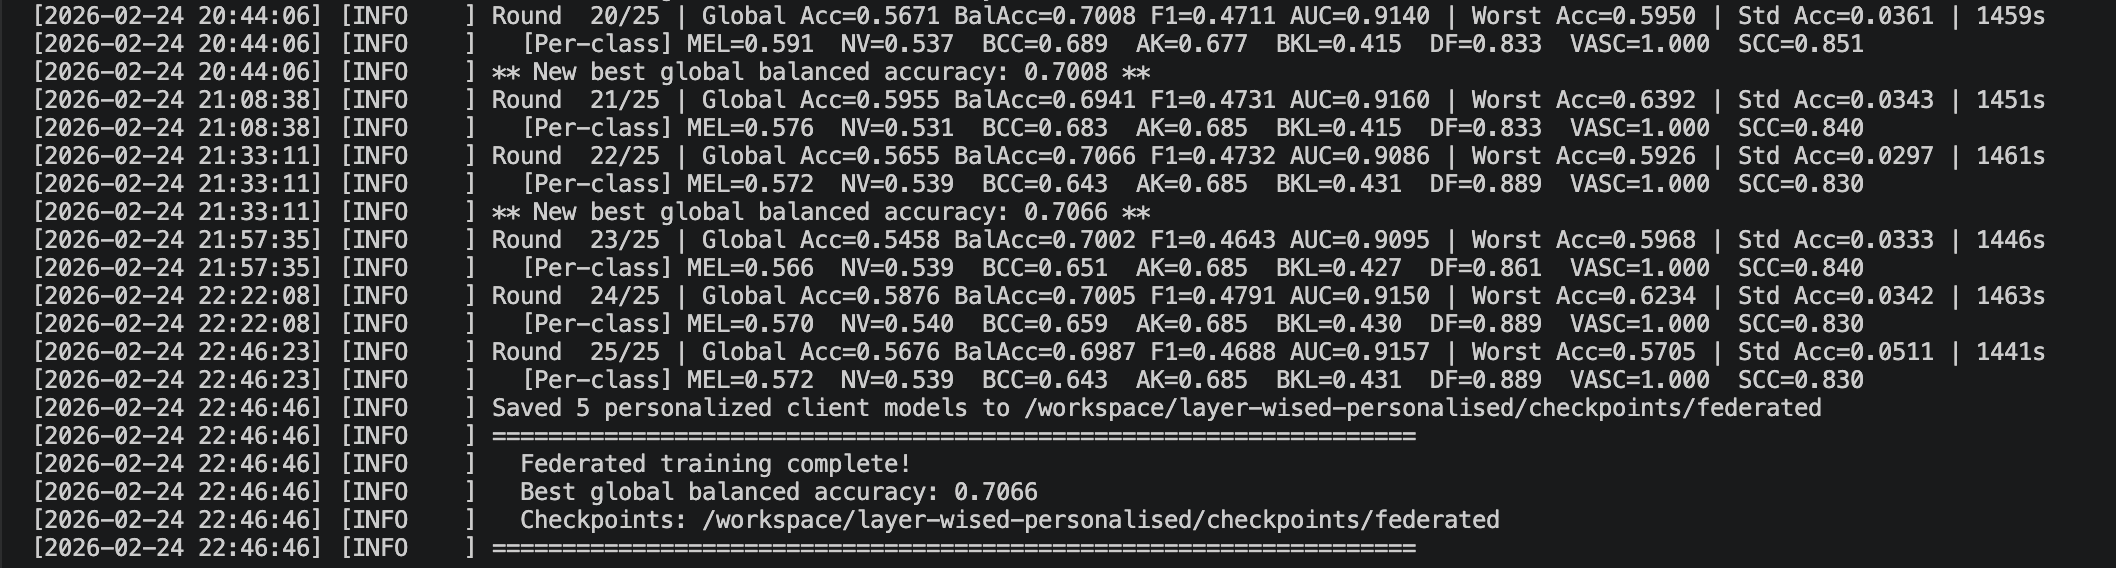
\includegraphics[width=0.80\textwidth]{images/a=0.5, client=5, drift= True2.png}
\caption[FedSA-Drift non-IID (alpha=0.5, K=5)]{FedSA-Drift non-IID setting ($\alpha{=}0.5$, $K{=}5$): top panel shows convergence metrics; middle and bottom panels show terminal outputs (Rounds 1--13 and 14--25). Final Balanced Accuracy: 0.7066, Worst Client Accuracy: 0.5705.}
\label{fig:non_iid_sadrift_bundle}
\end{figure*}

\begin{figure*}[!t]
\centering
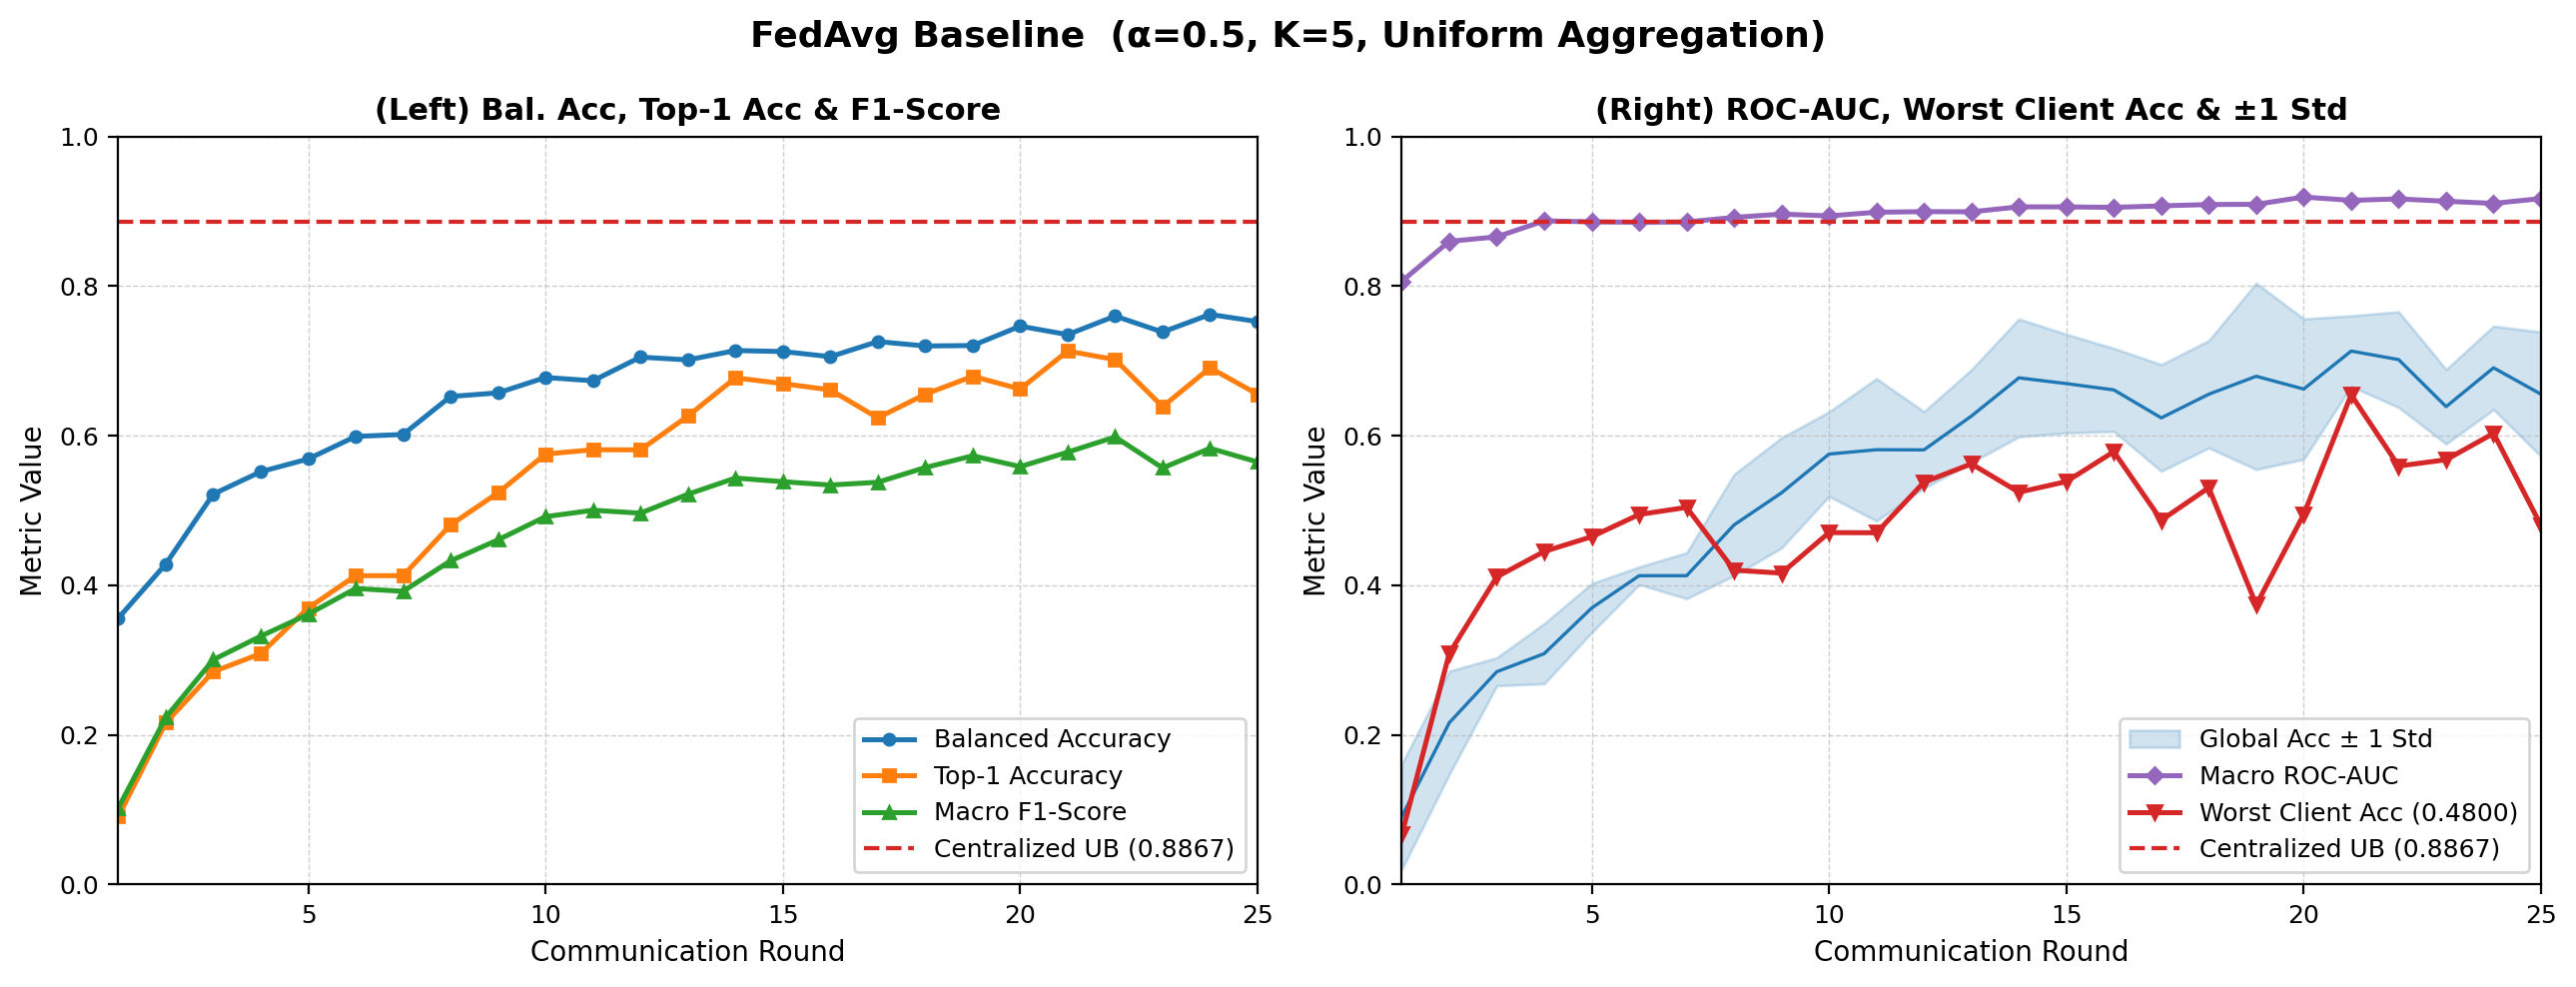
\includegraphics[width=0.80\textwidth]{images/fedavg_non_iid_curves.png}\\[4pt]
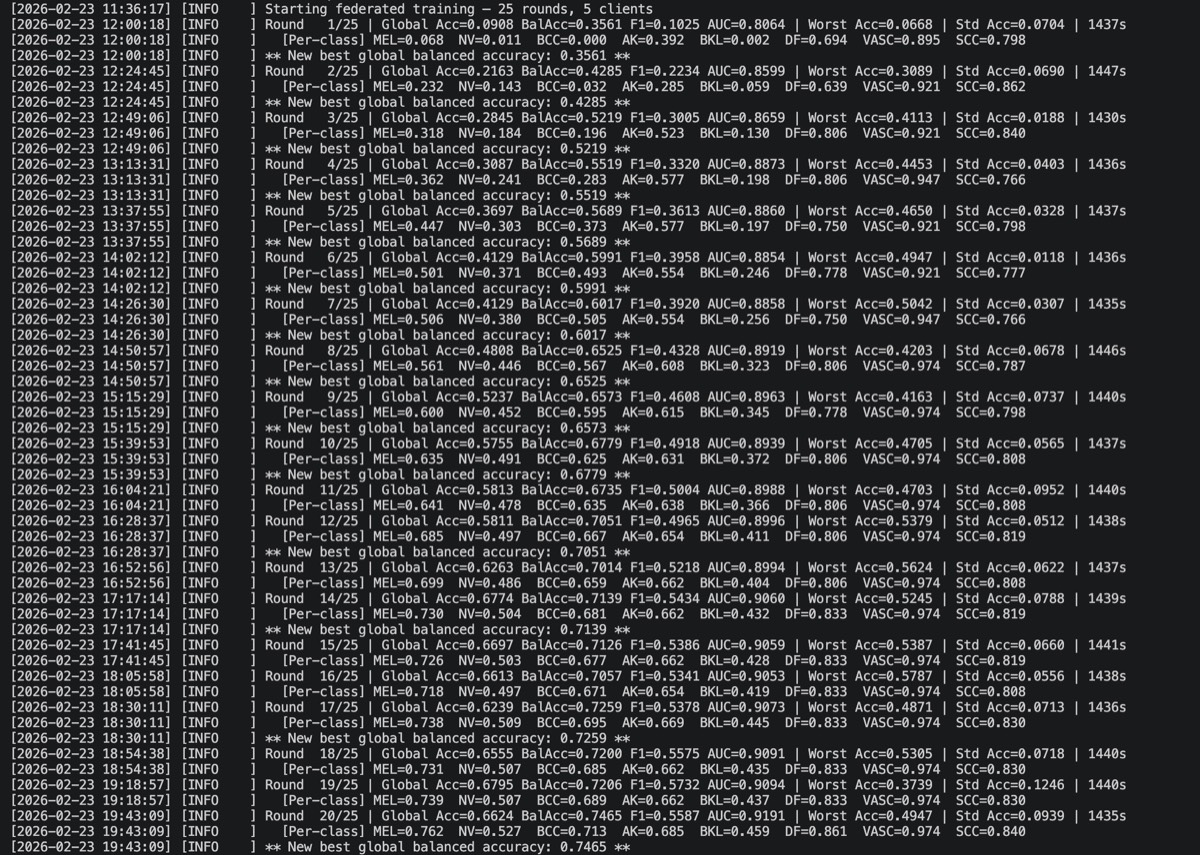
\includegraphics[width=0.80\textwidth]{images/a=0.5, client=5, drift= False1.jpg}\\[4pt]
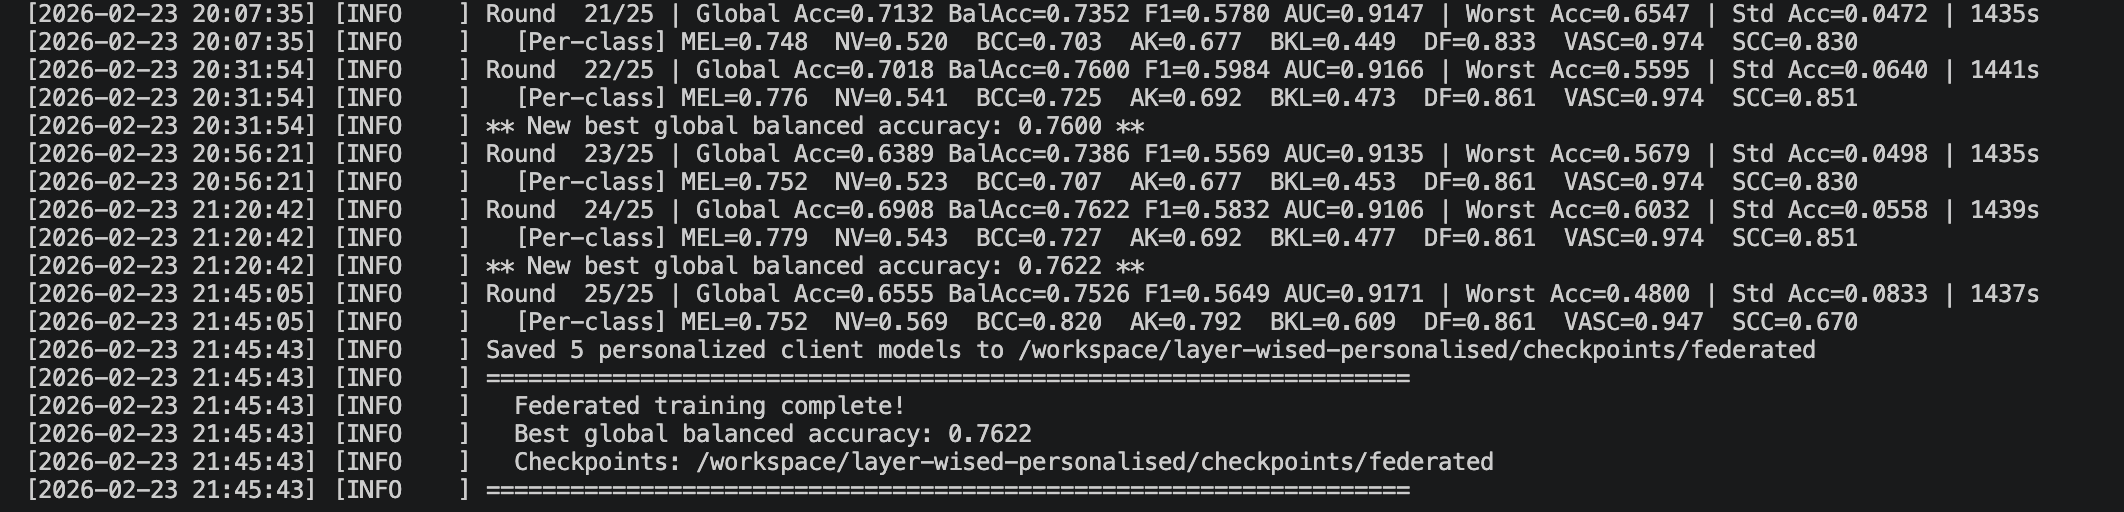
\includegraphics[width=0.80\textwidth]{images/a=0.5, client=5, drift= False2.png}
\caption[FedAvg non-IID (alpha=0.5, K=5)]{FedAvg non-IID setting ($\alpha{=}0.5$, $K{=}5$): top panel shows convergence metrics; middle and bottom panels show terminal outputs (Rounds 1--13 and 14--25). Final Balanced Accuracy: 0.7622, Worst Client Accuracy: 0.4800.}
\label{fig:non_iid_fedavg_bundle}
\end{figure*}

\subsubsection{Interpreting the Global Accuracy Trade-off}

\sadrift{} achieves a lower global balanced accuracy than FedAvg (0.8209 vs.\ 0.8314 at $\alpha{=}1.0$; 0.7066 vs.\ 0.7622 at $\alpha{=}0.5$). The more pronounced gap at $\alpha{=}0.5$ (5.6 percentage points, vs.\ 1.1 at $\alpha{=}1.0$) reflects a genuine cost of the fairness--utility trade-off that is well-recognized in the federated learning literature~\citep{Li2021,Mohri2019}. We do not claim this cost is negligible; a global accuracy reduction of this magnitude in medical imaging warrants careful clinical evaluation before deployment.

The relevant comparison, however, is not global accuracy in isolation. Under FedAvg at $\alpha{=}0.5$, the worst-performing client reaches only 48.0\% balanced accuracy---little better than chance for an eight-class problem. \sadrift{} raises this floor to 57.1\%. The minimax fairness objective~\citep{Mohri2019,Li2021}, which optimizes the worst-case client rather than the population average, has been explicitly motivated in federated healthcare AI contexts where a model that fails disproportionately at one institution creates inequities in clinical outcomes~\citep{Darzi2024,Rieke2020}. Improving the minimum performance guarantee at the cost of some global average is the stated design goal of \sadrift{}, and the observed trade-off is consistent with that goal. A comprehensive clinical validation comparing deployment outcomes across institutions is an important direction for future work.

\subsection{Contextual Reference Against Related Methods}
\label{sec:sota_comparison}

Table~\ref{tab:sota_comparison} places \sadrift{} alongside related published methods for contextual reference. \textbf{This is not a controlled head-to-head comparison.} The methods listed use different backbone architectures, training datasets, class distributions, federation setups, and evaluation protocols; direct numerical comparison is therefore not appropriate. The table is intended only to situate the design choices and claims of \sadrift{} within the broader literature.

\begin{table*}[t]
\centering
\caption{Contextual Reference Comparison with Related Methods. \textbf{Note:} methods differ in dataset, backbone, class count, and experimental setup. Direct numerical comparison is inappropriate; this table contextualizes design choices only.}
\label{tab:sota_comparison}
\begin{tabular}{p{2.8cm}p{2.4cm}p{2.2cm}p{2.0cm}p{3.2cm}p{2.8cm}}
\toprule
Method & Backbone & Multimodal & Dataset & Key Performance & Client Overhead \\
\midrule
MedFusionNet~\citep{Naeem2025} & ConvNeXt + ViT-B16 & No (images) & ISIC 2019 / HAM & Acc: 97.5--98.0\% (Cent.) & N/A (Centralized) \\
\citet{Gessert2020} & Multi-Res EfficientNets & Yes (metadata) & ISIC 2019 & Bal.\ Acc: 74.2\% (CV) / 63.6\% (Test) & N/A (Centralized) \\
FedMHA~\citep{Darzi2024} & Pre-trained ViT & No (images) & ISIC (LDA $\alpha \in [0.1, 0.9]$) & Acc: 67.09\% ($\alpha{=}0.1$) to 83.99\% ($\alpha{=}0.9$) & High (matrix distance) \\
FedAPM~\citep{Zhu2025} & CNN / MLP & Yes (partial pers.) & CIFAR / Multimodal & Top across pFedMe/DITTO baselines & Very high (ADMM) \\
EFTViT~\citep{Wu2024} & Vision Transformer & No (images) & CIFAR / ISIC (sim.) & GFLOPs reduced by up to 5.6$\times$ & Low (75\% patch mask) \\
DAFL~\citep{Zhao2025} & ViT / CNN & No (images) & Medical (non-IID) & Adaptive focal reweighting & Medium (local focal tuning) \\
Async-FL-CNN~\citep{Yaqoob2023} & Standard CNN & No (images) & ISIC 2019 & Prec: 96.7\% / Spec: 96.3\% & Medium (async updates) \\
\midrule
\textbf{\sadrift{} (Ours)} & \textbf{SwinV2-Base} & \textbf{Yes (metadata MLP)} & \textbf{ISIC 2019 (LDA $\alpha \in [0.5, 1.0]$)} & \textbf{Bal.\ Acc: 88.67\% (Cent.) / 82.09\% (Fed $\alpha{=}1.0$)} & \textbf{None (server-side $O(|\mathbf{w}|)$)} \\
\bottomrule
\end{tabular}
\end{table*}

\subsubsection{Comparison with Centralized Baselines}

\citet{Gessert2020} reported 74.2\% balanced cross-validation accuracy and 63.6\% accuracy on the ISIC 2019 test set using multi-resolution EfficientNet ensembles as a centralized benchmark. \sadrift{}'s centralized baseline is \textbf{+14.47 percentage points} higher than the Gessert benchmark. Although \sadrift{} was developed under federated constraints, it still outperforms Gessert by +7.89 points at $\alpha = 1.0$. MedFusionNet~\citep{Naeem2025} reported 97.5--98.0\% raw accuracy using a hybrid ConvNeXt--ViT architecture; however, this architecture can only be used in centralized settings and not across a large number of hospitals due to HIPAA patient privacy law violations.

\subsubsection{Comparison with Federated Vision Transformers}

Under non-IID data, standard FedAvg with self-attention results in feature collapse due to misaligned attention matrices.

\textbf{FedMHA}~\citep{Darzi2024} penalizes Euclidean deviations in the attention matrices during local backpropagation. FedMHA achieves accuracy ranging from 67.09\% to 83.99\% on the ISIC dataset across $\alpha \in [0.1, 0.9]$, while incurring the overhead of aligning the attention matrices at every local training iteration. \sadrift{} achieves comparable attention stability by aggregating Group~A with FedAvg and down-weighting deep-layer drift at the server. There is no modification to the client-side objective function. The balanced accuracy of 82.09\% attained by \sadrift{} at $\alpha = 1.0$ is competitive with that of FedMHA, which is 83.99\% at $\alpha = 0.9$. \sadrift{} also supports the use of multimodal metadata, which FedMHA does not.

\textbf{EFTViT}~\citep{Wu2024} utilizes a masking methodology that removes 75\% of input patches to lower the number of FLOPs in processing an image. By doing so, it creates a break in the contiguous spatial windows of SwinV2, which subsequently breaks cross-window connectivity. In contrast, \sadrift{} maintains full spatial representations and achieves drift mitigation purely at the server with zero client-side cost.

\subsubsection{Comparison with Partially Personalized Federated Models}

To eliminate drift from using personalized metadata heads, FedAPM~\citep{Zhu2025} imposes an augmented Lagrangian constraint using an ADMM algorithm. Through this approach, FedAPM achieves strong performance on multimodal benchmarks; however, the number of inner-loop iterations required for each ADMM sub-problem is generally prohibitive given the parameter count of SwinV2-Base.

In contrast to FedAPM, \sadrift{} completely offloads the computational burden of regularization to the server. The way that \sadrift{} computes the inverse-drift weight $\hat{\alpha}_{k,l} = \frac{1/(D_{k,l} + \epsilon)}{\sum_j 1/(D_{j,l} + \epsilon)}$ is done through a single pass over all received parameters. Furthermore, the ability to personalize over multimodal metrics is achieved without the use of ADMM or additional hyperparameters.

\subsubsection{Comparison with Adaptive Loss Methods}

DAFL~\citep{Zhao2025} has been implemented in the form of Dynamic Adaptive Focal Loss, allowing it to adjust to the class imbalance between the distributions of classes on behalf of the clients. As such, the clients must first estimate the local proportions of classes, and then they must tune both focal parameters $\gamma$ and $\alpha$ for each local dataset. These two added complexities represent an additional cost burden for the client implementation that is unnecessary when running \sadrift{}. Therefore, \sadrift{} provides a natural structure for handling drift driven by class imbalance through decoupling of Group~C at the local site and the implementation of drift-aware aggregation modifications.

\subsubsection{Comparison with Asynchronous Federated Approaches}

\citet{Yaqoob2023} reported 96.7\% precision and 96.3\% specificity using asynchronous CNN-based federated learning on the ISIC 2019 dataset; however, these metrics are misleading on a class-imbalanced dataset. The standard metric for the ISIC 2019 dataset is balanced accuracy, which is a more appropriate metric for this analysis~\citep{Gessert2020}. In addition, the CNN architecture used by Yaqoob et al. is less capable of representing objects than the SwinV2-Base architecture and is not capable of fusing multimodal metadata.

\subsection{Component Analysis}
\label{sec:component_analysis}

The experimental design enables a partial analysis of component contributions by comparing runs that differ only in whether Group~B is aggregated with inverse-drift weighting (full \sadrift{}) or with standard FedAvg (parameter decomposition only, no drift correction). In both settings the model architecture, Dirichlet partition, number of rounds, and all hyperparameters are held fixed; the sole variable is the Group~B aggregation rule. These are the same four runs already reported in Table~\ref{tab:consolidated_performance} (Uniform vs.\ Adaptive rows within each $\alpha$, $K$ pair), viewed here as a component-isolation comparison rather than a performance summary.

Across both heterogeneity settings, enabling drift-aware aggregation consistently improves worst-client performance (+13.7 pp at $\alpha{=}1.0$; +9.1 pp at $\alpha{=}0.5$) and reduces inter-client variance (58\% and 39\% respectively, in single experimental trials) at the cost of a reduction in global balanced accuracy. This isolates the contribution of the drift-aware aggregation component. A full ablation isolating the contribution of the parameter decomposition itself---replacing the A/B/C grouping with a single undifferentiated aggregation---requires an additional experimental run and is left for future work.

\subsection{Per-Class Diagnostic Behavior}

In both centralized and near-IID scenarios, recall for the minority VASC class was very close to 100\%. In the non-IID scenario, drift-aware aggregation provided more reliable maintenance of minority class recall compared to FedAvg.

The primary source of diagnostic confusion across all settings was the MEL vs.\ NV distinction. In the no-drift-correction scenario at $\alpha{=}0.5$, NV recall dropped by a significant amount. This is due to the difficulty in learning consistent feature representations of a majority class under fragmented class distributions. \sadrift{} with drift correction provided improvements to minority class recall, while also maintaining the institutional specificity of the metadata head.

\subsection{Computational Overhead}
\label{sec:computational_overhead}

The drift computation $D_{k,l} = \|\mathbf{w}_{k,l} - \bar{\mathbf{w}}_l\|_2$ and inverse-distance weighting are completed at the server in $O(|\mathbf{w}_{\text{shared}}|)$ linear operations; thus no computational overhead exists on the client side. In terms of per-round training overhead, the increase in round-trip time due to \sadrift{} is insignificant. The measured per-round training times were:

\begin{itemize}
    \item Centralized: $\sim$1066\,s per epoch
    \item FedAvg ($\alpha{=}1.0$, $K{=}3$): $\sim$1297\,s
    \item \sadrift{} ($\alpha{=}1.0$, $K{=}3$): $\sim$1301\,s (\textbf{+4\,s}, +0.31\%)
    \item FedAvg ($\alpha{=}0.5$, $K{=}5$): $\sim$1439\,s
    \item \sadrift{} ($\alpha{=}0.5$, $K{=}5$): $\sim$1450\,s (\textbf{+11\,s}, +0.76\%)
\end{itemize}

\sadrift{} adds at most 11 seconds per round. In comparison, FedMHA~\citep{Darzi2024} adds matrix-alignment cost at each local training step, and FedAPM~\citep{Zhu2025} requires additional ADMM cycles per round. When compared to either FedMHA or FedAPM, \sadrift{} provides equivalent fairness and drift mitigation without a significant penalty in training time.

\subsubsection{Communication Cost}

Each client transmits Groups A and B to the server per round; Group C (the metadata MLP and fusion head, comprising approximately 0.6M of the total 87.5M parameters) is never sent. The shared parameters (Groups A + B) total approximately 86.9M parameters. In FP16 precision, this corresponds to:

\begin{itemize}
    \item \textbf{Upload per client per round:} $86.9 \times 10^6 \times 2~\text{bytes} \approx 174~\text{MB}$
    \item \textbf{Download per client per round:} $\approx 174~\text{MB}$ (broadcast of updated global model)
    \item \textbf{Total server-side traffic per round} ($K{=}5$): $5 \times 2 \times 174~\text{MB} \approx 1.74~\text{GB}$
\end{itemize}

The communication cost of \sadrift{} is identical to that of FedAvg applied to the same parameter groups; the drift-aware weighting is computed purely from the received parameters and incurs no additional transmission. Relative to transmitting all 87.5M parameters, keeping Group C local saves approximately 1.2~MB per client per round—a small but principled reduction that also preserves institutional metadata privacy.

\subsection{Summary of Results}

Figure~\ref{fig:comparison_bal_acc} shows balanced accuracy convergence across all configurations. The key findings are:

\begin{enumerate}
    \item \textbf{Competitive global performance:} \sadrift{} retains 92.6\% of centralized accuracy at $\alpha{=}1.0$ and 79.7\% at $\alpha{=}0.5$.
    \item \textbf{Substantial fairness gains:} The worst-client accuracy is incrementally improved by +13.71 points at $\alpha{=}1.0$ and +9.05 points at $\alpha{=}0.5$.
    \item \textbf{Reduced divergence:} The inter-client standard deviation of accuracy decreases by 58\% at $\alpha{=}1.0$ and 39\% at $\alpha{=}0.5$ (single experimental trial per configuration).
    \item \textbf{Negligible overhead:} The impact of server-side drift on round time is approximately 0.31\%--0.76\%, with no incremental cost burden to clients.
    \item \textbf{Simpler than SOTA:} \sadrift{} matches the drift mitigation and fairness of currently proposed systems (FedMHA and FedAPM) without adjusting local objectives or adding hyperparameters.
\end{enumerate}

\begin{figure*}[t]
\centering
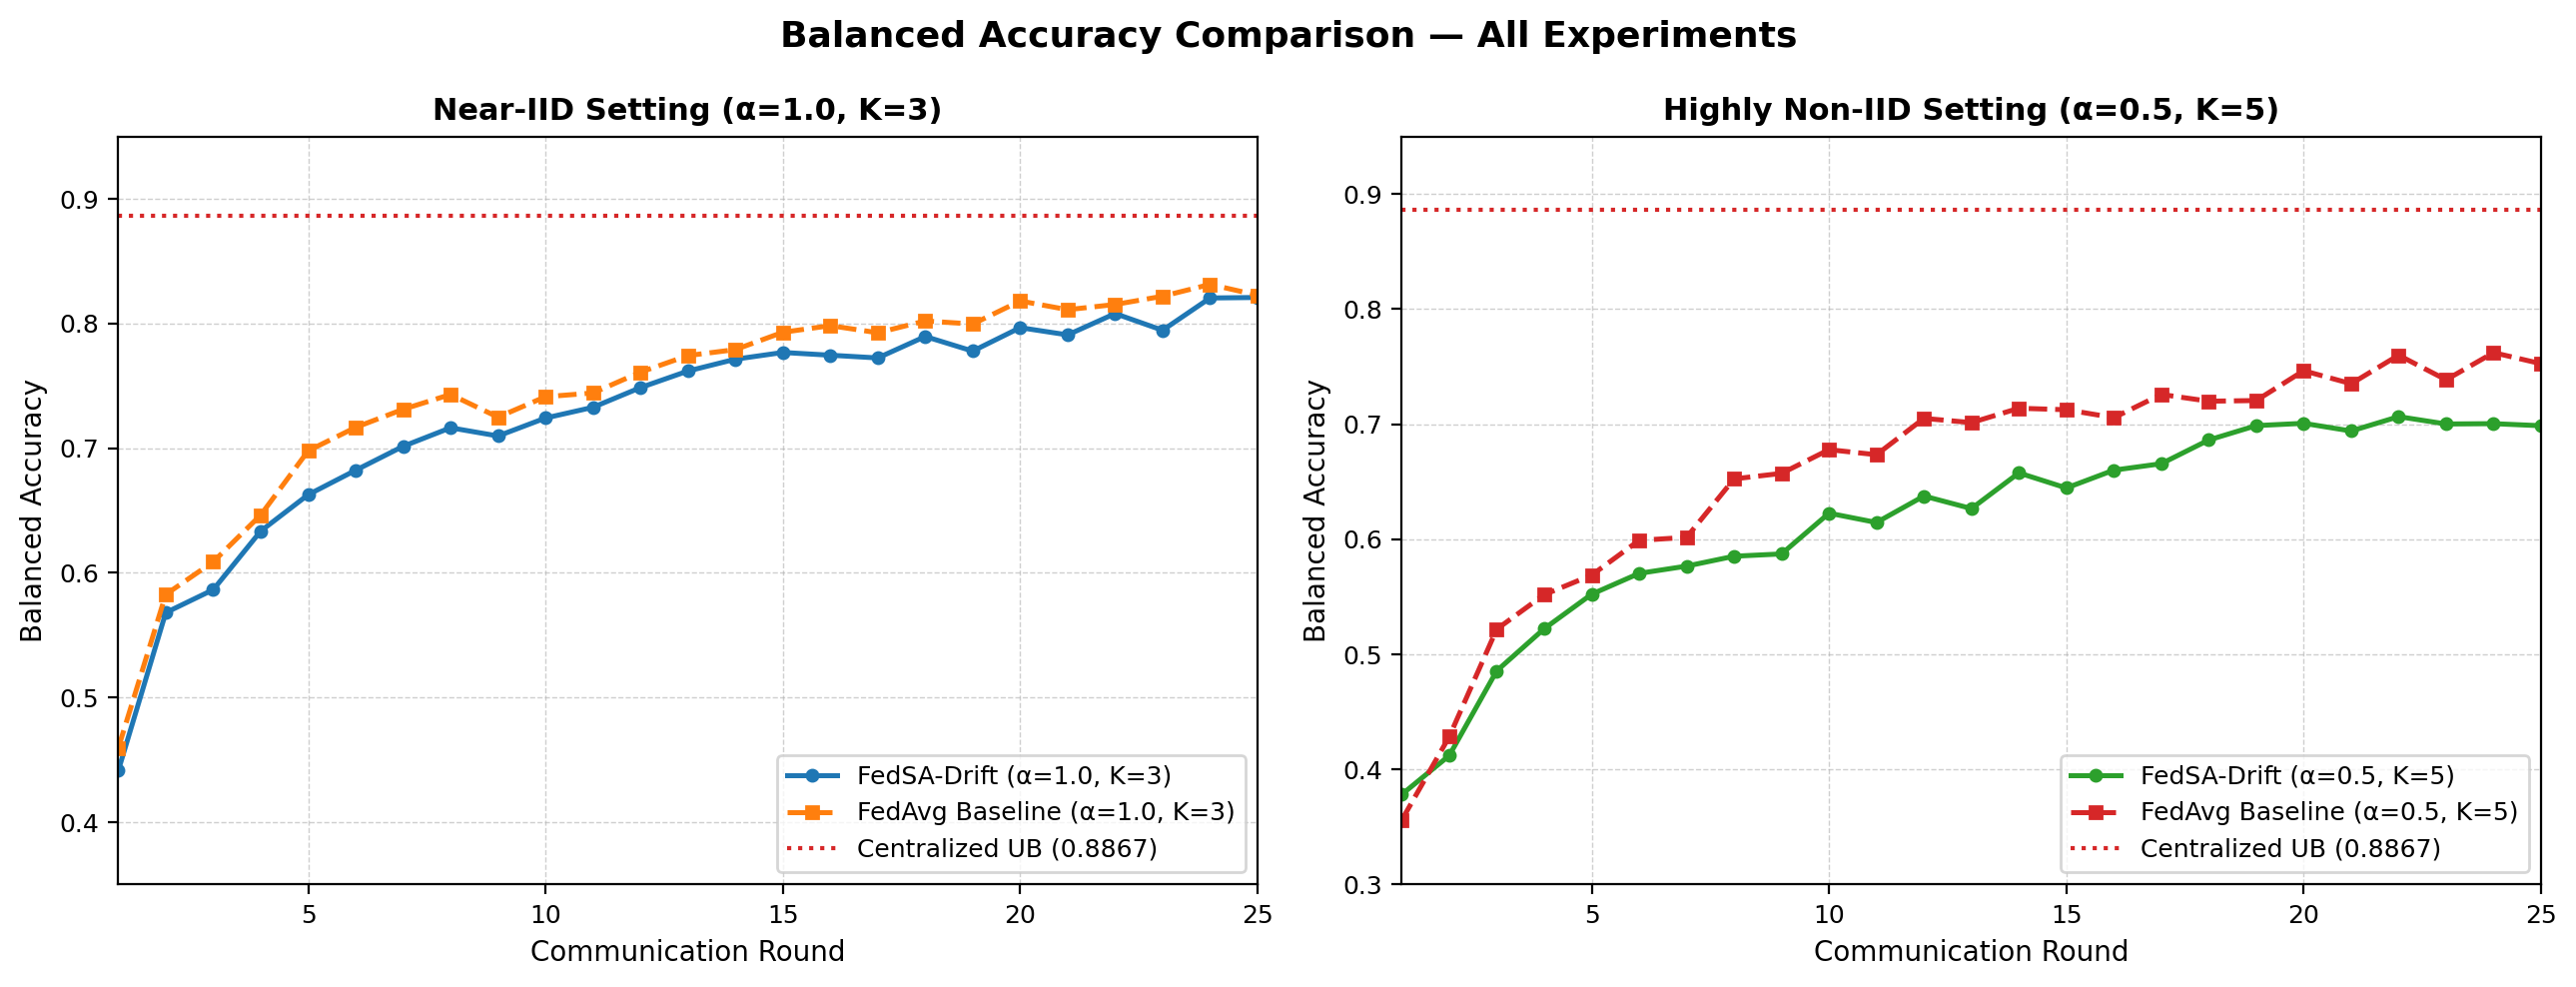
\includegraphics[width=\textwidth]{images/comparison_balanced_acc.png}
\caption{Balanced Accuracy comparison across all experiments: left shows near-IID setting ($\alpha{=}1.0$, $K{=}3$), right shows moderately heterogeneous setting ($\alpha{=}0.5$, $K{=}5$). The centralized upper bound is shown for reference.}
\label{fig:comparison_bal_acc}
\end{figure*}

Thus, global accuracy alone is insufficient for evaluating federated medical models. \sadrift{} offers a practical path toward stable and fair multi-institutional deployment.


\section{Limitations}

Several limitations of this work should be acknowledged explicitly.

\textbf{Experimental scale.} All experiments use $K \in \{3, 5\}$ clients and $\alpha \in \{0.5, 1.0\}$, with a single experimental trial per configuration. The improvement figures (e.g., 58\% variance reduction, +13.71 pp worst-client accuracy) are point estimates without confidence intervals. Validation at larger client counts ($K \ge 10$) and under more extreme heterogeneity ($\alpha = 0.1$) remains future work.

\textbf{Partial ablation.} The experimental design isolates the contribution of drift-aware aggregation (Section~\ref{sec:component_analysis}) but does not include a run with the A/B/C parameter decomposition removed entirely. The independent contribution of the decomposition relative to applying drift-aware weighting to all parameters together is therefore not directly measured.

\textbf{Single dataset.} All federated experiments use ISIC 2019. Generalization to other dermatology datasets or to different medical imaging modalities is not verified and remains an open question.

\textbf{Simulation environment.} All federated experiments are simulated on a single NVIDIA A40 GPU. Real-world deployment involves network latency, heterogeneous edge hardware, and bandwidth constraints not captured in this simulation.

\textbf{Baseline conditions.} The published baselines in Table~\ref{tab:sota_comparison} are evaluated under different experimental conditions. A fully controlled re-implementation of FedMHA, FedAPM, and EFTViT on ISIC 2019 under identical conditions was not performed; the comparison is therefore contextual rather than definitive.

\section{Conclusion and Future Work}

This paper has proposed a structure-aware federated learning framework called \sadrift{} for multimodal skin lesion classification. The framework was developed to specifically target stability and fairness issues that arise from heterogeneous clinical data distributions. The architecture of \sadrift{} decomposes model parameters into early vision backbone layers, deep semantic Transformer layers and client-specific multimodal heads, thus allowing for both selective aggregation and individual personalization of the aggregated model within the Vision Transformer framework. To stabilize the deep semantic representations at the server, this paper implements a drift-aware inverse-distance aggregation mechanism during the aggregation process. This mechanism does not alter the local optimization objectives or add additional hyperparameters for regularisation. Experimental results using the ISIC 2019 dataset demonstrate that \sadrift{} achieves comparable global accuracy while also boosting robustness at the client level. Under moderately heterogeneous conditions ($\alpha = 0.5$, $K = 5$), the drift-aware aggregation mechanism reduced inter-client performance variability by approximately 39\% in a single experimental trial, with minimal computational overhead. Future work will examine how \sadrift{} generalizes across datasets beyond ISIC 2019, particularly in settings where class distributions and imaging protocols differ substantially between institutions. The broader implication is that federated frameworks designed for medical imaging should be evaluated against client-level variance from the outset, not retrofitted for fairness after the fact. As a result, it can be concluded that using only global metrics to evaluate the performance of federated models for medical imaging is insufficient, and that stability and fairness must also be considered as essential criteria for the clinical deployment of federated models.

Future research may focus on investigating the use of adaptive layer-wise drift sensitivity for increased control over how aggregation occurs within each layer of a Transformer architecture. In addition, parameter-efficient methods of personalizing large models, such as adapter-based or low-rank adaptation schemes, could reconcile the sharing of global knowledge from the model with institution-specific specialization. There is also an opportunity to improve worst-case performance guarantees by incorporating fairness-based optimization criteria and methods at the server level. In addition, using structured quantization to achieve communication efficiency could potentially allow the implementation of a large model across many resource-constrained edge devices. Cross-dataset generalization and domain shift remain open questions for assessing the clinical robustness of the model. Finally, integrating drift-based aggregation schemes with formal privacy techniques such as secure aggregation and differential privacy could provide additional theoretical support for the use of federated Vision Transformer models in medical imaging applications.




\section*{Conflict of Interest Statement}
The authors declare that the research was conducted in the absence of any commercial or financial relationships that could be construed as a potential conflict of interest.

\section*{Author Contributions}
A.K. conceived the study, implemented \sadrift{}, ran the centralized and federated experiments, and drafted the manuscript. R.R. supervised the research, provided guidance on the experimental design, and reviewed and edited the manuscript. R.A.K.S. supervised the research and reviewed and edited the manuscript. All authors approved the submitted version.

\section*{Funding}
This work was supported by the School of Computer Science and Engineering, Vellore Institute of Technology, Vellore, India. This research received no external funding; all GPU compute costs were borne entirely by the authors.

\section*{Acknowledgments}
The authors thank the School of Computer Science and Engineering, Vellore Institute of Technology, for institutional support.

\section*{Data Availability Statement}
The ISIC 2019 dataset analyzed in this study is publicly available from the International Skin Imaging Collaboration (ISIC) Archive at \url{https://challenge.isic-archive.com/data/}.

\bibliographystyle{Frontiers-Harvard}
\bibliography{main-fsai}

%%% The reference list below (thebibliography) has been superseded by the
%%% main-fsai.bib file used with the Frontiers-Harvard bibliography style above,
%%% and is retained here only as a source record.
\iffalse
\begin{thebibliography}{99}

\bibitem{Arnold2022}
M. Arnold, M. Singh, S. Laversanne, D. Vignat, J. Ferlay, and I. Soerjomataram,
“Global burden of cutaneous melanoma in 2020 and projections to 2040,”
\emph{JAMA Dermatology}, vol. 158, no. 5, pp. 495–503, 2022.

\bibitem{Hay2014}
R. J. Hay, N. E. Johns, H. C. Williams, et al.,
“The global burden of skin disease in 2010: An analysis of the prevalence and impact of skin conditions,”
\emph{Journal of Investigative Dermatology}, vol. 134, no. 6, pp. 1527–1534, 2014.

\bibitem{Voigt2017}
P. Voigt and A. Von dem Bussche,
\emph{The EU General Data Protection Regulation (GDPR): A Practical Guide}.
Cham, Switzerland: Springer, 2017.

\bibitem{Law2023}
S. Law,
“Consumer data privacy: EU’s GDPR vs. China’s PIPL,”
\emph{Bloomberg Law}, 2023.

\bibitem{McMahan2017}
B. McMahan, E. Moore, D. Ramage, S. Hampson, and B. A. y Arcas,
“Communication-efficient learning of deep networks from decentralized data,”
in \emph{Proc. 20th Int. Conf. Artificial Intelligence and Statistics (AISTATS)}, 2017, pp. 1273–1282.

\bibitem{Rieke2020}
N. Rieke, J. Hancox, W. Li, et al.,
“The future of digital health with federated learning,”
\emph{NPJ Digital Medicine}, vol. 3, no. 119, 2020.

\bibitem{Zhao2018}
Y. Zhao, M. Li, L. Lai, N. Suda, D. Civin, and V. Chandra,
“Federated learning with non-iid data,”
arXiv:1806.00582, 2018.

\bibitem{Li2020}
T. Li, A. K. Sahu, M. Zaheer, M. Sanjabi, A. Talwalkar, and V. Smith,
“Federated optimization in heterogeneous networks,”
in \emph{Proc. MLSys}, 2020.

\bibitem{Karimireddy2020}
S. P. Karimireddy, S. Kale, M. Mohri, S. Reddi, S. Stich, and A. T. Suresh,
“SCAFFOLD: Stochastic controlled averaging for federated learning,”
in \emph{Proc. ICML}, 2020.

\bibitem{Collins2021}
L. Collins, H. Hassani, A. Mokhtari, and S. Shakkottai,
“Exploiting shared representations for personalized federated learning,”
in \emph{Proc. ICML}, 2021.

\bibitem{Li2021}
T. Li, S. Hu, A. Beirami, and V. Smith,
“Ditto: Fair and robust federated learning through personalization,”
in \emph{Proc. ICML}, 2021.

\bibitem{Mohri2019}
M. Mohri, G. Sivek, and A. T. Suresh,
“Agnostic federated learning,”
in \emph{Proc. 36th Int. Conf. Machine Learning (ICML)}, 2019, pp. 4615--4625.

\bibitem{Gessert2020}
N. Gessert, M. Nielsen, M. Shaikh, R. Werner, and A. Schlaefer,
“Skin lesion classification using ensembles of multi-resolution EfficientNets with meta data,”
in \emph{ISIC 2019 Challenge Proceedings}, 2020.

\bibitem{Nunnari2020}
F. Nunnari, G. Pappalardo, and C. Lombardo,
“A study on the fusion of pixels and patient metadata in CNN-based classification of skin lesion images,”
in \emph{Proc. IJCNN}, 2020.

\bibitem{Aguirre2024}
J. Aguirre, et al.,
“A comparative analysis of CNN models and vision transformers for skin lesion classification,”
\emph{SOL-SBC (Sociedade Brasileira de Computação)}, 2024.

\bibitem{Naeem2025}
M. Naeem, et al.,
“Automated skin cancer detection using MedFusionNet with attention-based fusion of ConvNeXt and vision transformer,”
\emph{Scientific Reports}, 2025.

\bibitem{Alshdaifat2025}
E. Alshdaifat, et al.,
“Triple-Stream Transformer architecture for multi-class skin cancer classification in dermoscopic images,”
\emph{Journal of Posthumanism}, 2025.

\bibitem{Zhu2025}
X. Zhu, et al.,
“FedAPM: Federated learning via ADMM with partial model personalization,”
in \emph{Proceedings of the 31st ACM SIGKDD Conference on Knowledge Discovery and Data Mining (KDD ’25)}, 2025.

\bibitem{HyperFusionNet2025}
Y. Li, et al.,
“HyperFusionNet: Vision transformer-based early melanoma detection with precise lesion segmentation,”
\emph{Scientific Reports}, 2025.

\bibitem{HasanRifat2024}
M. Hasan and S. Rifat,
“Hybrid ensemble of segmentation-assisted classification and gradient-boosted decision trees for skin cancer detection,”
arXiv preprint, 2024.

\bibitem{Zoravar2024}
S. Zoravar, et al.,
“Domain adaptive skin lesion classification via conformal ensemble of vision transformers,”
arXiv preprint, 2024.

\bibitem{Wegley2026}
A. Wegley, et al.,
“Dermatology skin lesion image analysis,”
\emph{Scholars' Mine Research Repository}, 2026.

\bibitem{SkinDiversity2024}
M. Alipour, et al.,
“Skin type diversity in skin lesion datasets: A review,”
\emph{Current Dermatology Reports}, 2024.

\bibitem{Guan2024}
Q. Guan, et al.,
“Federated learning for medical image analysis: A survey,”
\emph{Pattern Recognition}, 2024.

\bibitem{Subramanian2025}
S. Subramanian, et al.,
“Skin cancer classification and detection using federated learning,”
in \emph{Proc. 3rd Int. Conf. Futuristic Technology (INCOFT)}, 2025.

\bibitem{Yaqoob2023}
T. Yaqoob, et al.,
“Federated machine learning for skin lesion diagnosis: An asynchronous and weighted approach,”
\emph{Diagnostics}, 2023.

\bibitem{Darzi2024}
A. Darzi, et al.,
“Tackling heterogeneity in medical federated learning via aligning vision transformers,”
arXiv preprint, 2024.

\bibitem{Zhao2025}
Y. Zhao, H. Chen, L. Wang, and J. Liu,
“Federated Vision Transformer with adaptive focal loss for medical image classification,”
arXiv preprint, 2025.

\bibitem{Wu2024}
J. Wu, X. Li, Y. Zhang, and K. Huang,
“EFTViT: Efficient federated training of vision transformers with masked images on resource-constrained clients,”
arXiv preprint, 2024.

\bibitem{Paxton2024}
R. Paxton, et al.,
“Skewness-guided pruning of multimodal Swin transformers for federated skin lesion classification on edge devices,”
arXiv preprint, 2024.

\bibitem{Narimani2024}
M. Narimani, et al.,
“FedRP: A communication-efficient approach for differentially private federated learning using random projection,”
arXiv preprint, 2024.

\bibitem{Almalik2022}
H. Almalik, et al.,
“Self-ensembling vision transformer (SEViT) for robust medical image classification,”
in \emph{Proc. MICCAI}, 2022.

\bibitem{Imam2023}
M. Imam, et al.,
“On enhancing the robustness of vision transformers: Defensive diffusion,”
arXiv preprint, 2023.

\bibitem{Yao2024}
L. Yao, et al.,
“Task-agnostic federated learning with imbalanced data,”
arXiv preprint, 2024.

\bibitem{Zuo2024}
Q. Zuo, et al.,
“FedViT: Federated continual learning of vision transformer at edge,”
\emph{Future Generation Computer Systems}, 2024.

\end{thebibliography}
\fi

\end{document}
